\chapter{Protocole expérimental général}
\mylocaltoc


\section{Introduction du chapitre}\label{chap:IntroProtocExp}
Après avoir brièvement rappelé les bases de fonctionnement des machines thermoacoustiques, il est temps de décrire le réfrigérateur support de cette thèse. 

Le choix de la géométrie, les paramètres hydrauliques du régénérateur utilisé, et enfin la chaîne d'excitation et d'acquisition sont présentés dans la section~\ref{chap:PresentationTacot} (\nameref{chap:PresentationTacot}). La deuxième partie présente les conditions expérimentales choisies ainsi que le protocole suivi pour chaque mesure dans la section~\ref{chap:ProtocolExpe} (\nameref{chap:ProtocolExpe}). Les simulations théoriques réalisées sont ensuite expliquées en troisième partie, dans la section~\ref{chap:SimusRealisees} (\nameref{chap:SimusRealisees}).

Ces parties visent à créer une vue d'ensemble de ce qui est fait durant cette thèse et le présenter de manière globale pour pouvoir s'y référer dans les différents chapitres suivants.

\section{Présentation du dispositif expérimental actuel}\label{chap:PresentationTacot}
\subsection{Géométrie du réfrigérateur \textsc{Tacot}}
\subsubsection{Cavité thermoacoustique}
La pompe à chaleur a été dimensionnée et fabriquée dans le cadre du projet ANR \textsc{Tacot} (ThermoAcoustic Cooler for Onroad Transportation), qui porte sur l'application d'une pompe à chaleur thermoacoustique pour la climatisation automobile \cite{ANR_thermo-acoustic_2019}. Ce projet apporte beaucoup de contraintes, dont l'une des principales est la compacité. Contrairement aux autres systèmes thermoacoustiques existant et bien plus volumineux (tels que le liquéfacteur de gaz naturel développé par Swift et Wollan au Los Alamos National Laboratory \cite{swift_thermoacoustics_2002, wollan_development_2002}, ou le réfrigérateur cryogénique thermoacoustique spatial (STAR) \cite{adeff_measurement_1991, garrett_thermoacoustic_1993}, ou encore), les dimensions doivent être réduites tout en conservant un pompage de chaleur efficace. Pour cela, une géométrie coaxiale pour la cavité thermoacoustique est préférée à celle toroïdale usuellement utilisée en suivant les travaux de Poignand et al. \cite{poignand_thermoacoustic_2011, poignand_analysis_2013}. L'ajout d'une source acoustique secondaire dans la cavité thermoacoustique permet également de gagner en compacité, en remplaçant un résonateur plus long par la masse de son équipage mobile et la souplesse de sa suspension, tel que réalisé dans les travaux de Poese et al. \cite{poese_thermoacoustic_2004}. De plus, la présence de cette source assure le déphasage optimal entre pression et vitesse acoustiques au sein du noyau thermoacoustique. Un schéma général présente la géométrie de la pompe à chaleur sur la figure~\ref{fig:SchemaGeneralTACOT}, adapté de Ramadan et al. \cite{ramadan_design_2021}.


\begin{figure}[!ht]
    \centering
    \external{fig_SchemaGeneralTACOT}
%    \externalremake
    \begin{tikzpicture}[scale=.5]
	\node[anchor=south west, inner sep=0] (image) at (0,0) {\includegraphics[angle=0,origin=c,width=.6\textwidth]{../fig/fig_TACOTSchematics/TACOT.png}};
	
	\node[anchor=east, inner sep=0] (imagecropped) at (image.west) {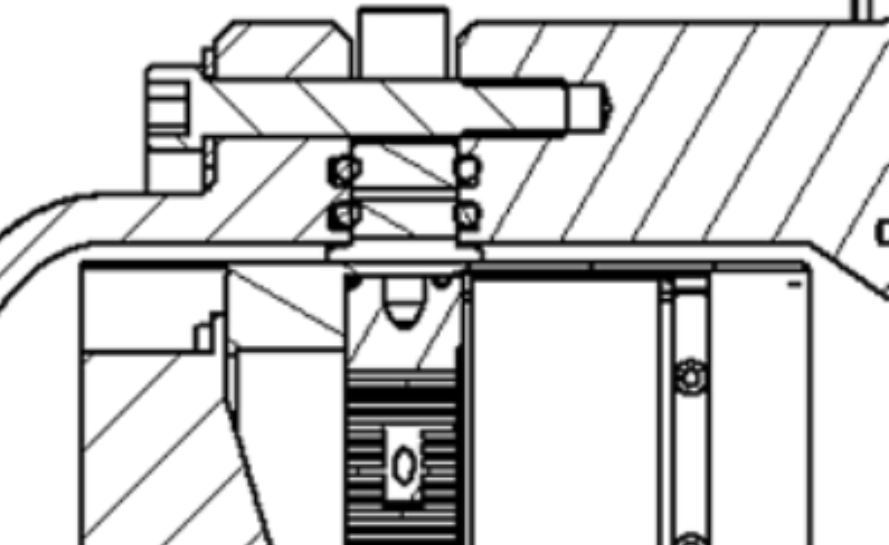
\includegraphics[angle=0,origin=c,width=.35\textwidth]{../fig/fig_TACOTSchematics/TACOT_Cropped.png}};

\draw[black, very thick, dashed, rounded corners] (imagecropped.north west) rectangle (imagecropped.south east);
%\draw[black, very thick, dashed, rounded corners] ($(AHX)+(-1.5cm,3cm)$) rectangle ($(CHX)+(.75cm,-.5cm)$);
	
	\begin{scope}[x={(image.south east)},y={(image.north west)}]
	
%		\filldraw (0,0) circle (2pt); 
%		\filldraw[green] (1,0) circle (1pt);
%		\filldraw[red] (1,1) circle (1pt);		
%		\filldraw[blue] (0,1) circle (1pt);
%		\draw[help lines,xstep=.1,ystep=.1] (0,0) grid (1,1);
%		\fill[orange, rounded corners, opacity=1,draw=orange] (.46,.65) -- ++(132:.09) -- ++(0,-.44) -- ++(48:.09) -- cycle;
		\draw[MatlabYellow,rounded corners,very thick,preaction={fill=MatlabYellow!20,opacity=.5}] (.46,.65) -- ++(132:.09) -- ++(-.03,0) -- ++(0,-.44) --++(.03,0) -- ++(48:.09) -- cycle; %node[left,pos=.5,label={[rotate=90]center:Cavité}]{};
		\draw[MatlabYellow] (.415,0.5) node [label={[rotate=90]center:\textbf{Cône}}]{};
		
%		\draw[blue] (.5,.5) node [anchor=center, preaction={fill=black!20,opacity=.7}] {RIX};
%		\draw[red] (.33,.5) node [anchor=center, preaction={fill=black!20,opacity=.7}] {TA core};	
	
		\draw[MatlabPurple,rounded corners,very thick,preaction={fill=MatlabPurple!20,opacity=.5}] (.365,.7) rectangle (.245,.3) node[pos=.5,label={[rotate=90]center:\textbf{Noyau}}]{};
		
		\node (AHX) at (.27,.65) {};
		\node (Reg) at (.32,.65) {};
		\node (CHX) at (.36,.65) {};
		\node (RIX) at (.77,.4) {};

		\node (HP) at (.19,.4) {};
		
		\draw[<-,very thick,MatlabOrange] (AHX.center) to[out=90,in=0] ($(AHX)+(-.2,.41)$) node[left]{\begin{tabular}{r} Echangeur de chaleur ambiant \\ (HXA) \end{tabular}};		
		\draw[<-,very thick] (Reg.center) to ($(Reg)+(0,.4)$) node[above]{Régénérateur};
		\draw[<-,very thick,MatlabBlue] (CHX.center) to[out=90,in=180] ($(CHX)+(.2,.41)$) node[right]{\begin{tabular}{l} Echangeur de chaleur froid \\ (HXF) \end{tabular}};
		
		\draw[->,very thick,green!50!black] ($(RIX)+(0,-.4)$) -- (RIX.center) node[pos=0,anchor=north]{\begin{tabular}{c}Source acoustique principale \\ (SA1) \end{tabular}};
		\draw[->,very thick,green!50!black] ($(HP)+(0,-.4)$) -- (HP.center) node (SA2) [pos=0,anchor=north]{\begin{tabular}{c}Source acoustique secondaire \\ (SA2) \end{tabular}};
		
%		\draw [white] (.455,.5) node{+};
%		\draw [white] (.41,.65) node{+};
%		\draw [white] (.41,.5) node{+};
%		\draw [white] (.41,.35) node{+};

		\draw[black, very thick, dashed, rounded corners] ($(AHX)+(-.14,.2)$) node(a){} rectangle ($(CHX)+(.07,-.1)$);
		
		\draw[black, very thick, dashed] (a) -- (imagecropped.north east);
		\draw[black, very thick, dashed] ($(a)+(0,-.3)$) -- (imagecropped.south east);
		

	\end{scope}
	
	\draw(imagecropped.south) node[below]{\small \textbf{(a)}};		
	\draw(SA2.south -| image.south) node{\small \textbf{(b)}};
	
\end{tikzpicture}
    \caption[Schéma général du réfrigérateur \textsc{Tacot} et mise en évidence des zones d'intérêt pour cette thèse]{Schéma général du réfrigérateur \textsc{Tacot}. Les \colorbox{MatlabYellow}{volume d'adapatation d'impédance} et \colorbox{MatlabOrange}{noyau thermoacoustique}, zones d'intérêt, sont mises en évidence.}
    \label{fig:SchemaGeneralTACOT}
\end{figure}



\subsubsection{Noyau thermoacoustique}
Tout comme la machine qui le contient, le noyau adopte une géométrie cylindrique et est composé d'un régénérateur encadré par deux échangeurs de chaleur. Les axes $\mathbf e_x$ et $\mathbf e_r$ sont alors respectivement définis dans les direction axiale et radiale du noyau, avec pour direction positive choisie dans le sens de l'échangeur froid vers l'échangeur ambiant pour le premier, et du centre du noyau vers l'extérieur pour le second.\medskip

Le régénérateur est composé de tissus métalliques (Gantois, modèle : 102045) empilés dans une enceinte cylindrique de diamètre intérieur $D_{\sf reg}=\qty{148}{\mm}$ et de longueur $L_{\sf reg}=\qty{39}{\mm}$ pour atteindre une porosité $\phi$ souhaitée et définie par 

\begin{align}
	\phi &= \frac{V_{\sf gaz}}{V_{\sf tot}}, \label{eq:Porosite_Volume}%\\
%	&= \frac{V_{\sf tot}-V_{\sf metal}}{V_{\sf tot}} \nonumber\\
%	&= 1 - \frac{m_{\sf metal}}{m_{\sf tot}} \label{eq:Porosite_Masse}
\end{align}
où $V_{\sf gaz}$ représente le volume occupé par le gaz dans le régénérateur, et $V_{\sf tot}$ le volume total du régénérateur. Le matériau est poreux et tortueux, et le rayon hydraulique est alors défini par \cite{swift_thermoacoustics_2017} %\echaf{ajouter source pour justifier que les matériaux type "mousse" se comporte comme du cylindrique : UPDATE dans Swift TA unifying... chapitre 7 (tortuous porous media)}

\begin{equation}
	r_h = d_w\frac{\phi}{4(1-\phi)},
	\label{eq:DefRayonHydrauGantois}
\end{equation}
avec $d_w$ le diamètre du fil. Les dimensions et paramètres du régénérateur sont résumés dans le tableau \ref{tab:ParamHydrauTAC}.

\begin{table}[!ht]
    \centering
    \begin{tabular}{l@{\hspace{1cm}}l}
    	\hline
    	\textbf{Paramètre [unité]} & \textbf{Valeur} \\\hline\hline
    	Diamètre du noyau $D_{\sf reg}$ [\unit{\meter}] & \num{148e-3} \\
    	Longueur du régénérateur $L_{\sf reg}$ [\unit{\meter}] & \num{39e-3} \\
    	Diamètre du fil $d_w$ [\unit{\meter}] & \num{53e-6} \\
        Rayon hydraulique $r_h$ [\unit{\meter}] & \num{2.81e-5} \\
        Porosité du noyau $\Phi$ [\unit{\percent}] & \num{68}\\
        Couche limite thermique $\delta_\kappa$ [\unit{\meter}] & \num{1.4452e-4} \\
        Couche limite visqueuse $\delta_\nu$ [\unit{\meter}] & \num{9.1120e-5} \\
        \echaf{Perméabilité} [\unit{\meter\squared}] & \\
        \hline
    \end{tabular}
    \caption{Paramètres hydrauliques du régénérateur à la fréquence de fonctionnement, \linebreak $f=\qty{47}{\Hz}$}
    \label{tab:ParamHydrauTAC}
\end{table}

Cette machine nécessite entre autres choses le respect de la condition $\delta_{\kappa,\nu} \gg r_h$, de sorte à avoir un excellent contact thermique entre le fluide et le solide poreux. Pour le fluide considéré, les épaisseurs de couches limites sont tracées en fonction de la fréquence et comparé au rayon hydraulique sur la figure~\ref{fig:dKdV}.

\begin{figure}[!ht]
    \centering
    \external{fig_dKdV}
%    \externalremake
    \begin{tikzpicture}
    \def\width{.9*\textwidth};
    \def\height{.45*\width};
    \def\spx{.25cm};
    \def\spy{1.25cm};
    \def\legx{.5cm};
    \def\legy{\legx};
    \def\prop{.45};
    \def\xcursor{47};
    \def\ycursorV{9.112e-5};
    \def\ycursorK{1.4452e-4};
    \def\rh{2.81e-5};
    
    \begin{axis}[name=dKdV,width={\width},height={\height},
    grid=both, minor tick num=10, 
    grid style={line width=.1pt, draw=gray!10},
    major grid style={line width=.2pt,draw=gray!50},
    xlabel={Fréquence $f$ [\unit{\Hz}]},
    ylabel={\'Epaisseurs de couches limites $\delta_{\kappa,\nu}$ [\unit{\m}]},
    xmin=0,xmax=75,ymin=0,ymax=.5/1000,
    xtick={0,25,50,75,100},
    extra x ticks={47},
    extra x tick style={
        grid=major,
        xticklabel={\num{47}},
        xticklabel style={yshift=0, anchor=north}
        },
    extra y ticks={\rh},
    extra y tick style={
        grid=major,
        yticklabel={$r_h$},
        yticklabel style={yshift=1mm, anchor=east}
        },
    ytick={0,1e-4,...,10e-4},
%    ytick={0,2.81/100000,9.1120/100000,1.4452/10000,
%    	2.5/10000,5/10000,1/1000},
    scaled y ticks = false,
    domain=0:100,
    legend cell align={left},
    legend style = {at={($(1,1)+(-2mm,-2mm)$)},anchor = north east,rounded corners}
    ]
        \addplot[solid,ultra thick,draw=Plasma1] file {../fig/fig_dKdV/data/data_dK.txt};
        \addplot[solid,ultra thick,draw=Plasma64] file {../fig/fig_dKdV/data/data_dV.txt};
        \filldraw[Plasma1] (\xcursor,\ycursorK) circle (2pt) node[above right]{$\delta_\kappa=\qty{\ycursorK}{\meter}$};
        \filldraw[Plasma64] (\xcursor,\ycursorV) circle (2pt) node[below left]{$\delta_\nu=\qty{\ycursorV}{\meter}$};
%        \draw[dashed,black!50] (\xcursor,0) -- (\xcursor,\ycursorK);
%        \draw[dashed,Plasma33] (\xcursor,\ycursorK) -- (0,\ycursorK) node[left]{\num{1.4452e-4}};
%        \draw[dashed,Plasma66] (\xcursor,\ycursorV) -- (0,\ycursorV) node[left]{\num{9.1120e-5}};
%         \draw[dashed,black!50] ({axis cs:\xcursor,0}|-{rel axis cs:0,0}) -- ({axis cs:\xcursor,0}|-{rel axis cs:0,\ycursorK});
       \addplot[loosely dashed,draw=black, ultra thick] {\rh};
       \draw(0,\rh) node[above right]{\qty{\rh}{\meter}};
        
        \legend{$\delta_\kappa$ \\ $\delta_\nu$ \\ $r_h$ \\};
    \end{axis}
\end{tikzpicture}
    \caption{\'Evolution des épaisseurs de couches limites thermique et visqueuse en fonction de la fréquence, définies par le système d'équations~\eqref{eq:CouchesLimites}.}
    \label{fig:dKdV}
\end{figure}



\subsection{Chaîne d'excitation et d'acquisition}
L'instrumentation utilisée est basée sur celle conçue au début du projet \cite{ramadan_design_2021}, tout en modifiant quelques éléments.

Premièrement, la chaîne d'excitation est présentée. Elle est assez simple, et se compose d'un générateur de fonction à deux canaux (TekTronix AFG3022). Chaque canal est ensuite connecté à un amplificateur pour chaque source acoustique. La source principale (RIX Industries, 1S241M) est alimentée par un amplificateur QSC PLD4.5, et la source secondaire (Peerless, GBS135F) par un amplificateur Yamaha P3500S.\medskip

%Un générateur basse fréquence génère les signaux d'alimentation des sources acoustiques. Il dispose de deux sorties, chacune connectée à un amplificateur avant d'être reliée aux transducteurs. Dans le cas de la source principale (RIX Industries, 1S241M), l'amplificateur est un QSC PLD4.5 tandis que pour la source secondaire (Peerless, GBS135F) il s'agit d'un Yamaha P3500S.

Ensuite, la chaîne d'acquisition se compose de plus de trente capteurs. Tous ne sont pas utilisés, mais peuvent servir de contrôle durant une expérience, pour s'assurer du bon déroulement de celle-ci.

\paragraph*{Alimentation électrique des sources} L'alimentation électrique de la source acoustique principale est mesurée au moyen d'une sonde différentielle \echaf{et le courant ?}

\paragraph*{Température} Dix-neuf thermocouples Type K de \qty{.5}{\milli\meter} de diamètre sont placés de la manière suivante : quinze thermocouples mesurent la température en différentes positions du noyau, un devant la source acoustique principale, deux derrière celle-ci, et un derrière la source acoustique secondaire. La carte d'acquisition utilisée (National Instruments, NI9213) ne comporte que seize entrées, et pour toutes les mesures ce sont les thermocouples du noyau et de devant la source acoustique principale qui y sont connectés. Le placement de ces thermocouples d'intérêt est représenté sur la figure~\ref{fig:TCdansNoyau} par les symboles `\textcolor{cyan}{\textbullet}'.

\begin{figure}[!ht]
    \centering
    \external{fig_TCdansNoyau}
    %\externalremake
    \begin{tikzpicture}[scale=.2]
	\def\rCHX{14cm};
	\def\lCHX{.7cm};
	\def\rREG{14.8cm};
	\def\lREG{3.9cm};
	\def\rAHX{11cm};
	\def\lAHX{2.3cm};
	
	
	\fill[pattern=horizontal lines,pattern color=MatlabOrange,draw=black] (0,-\rAHX) rectangle ++(\lAHX,2*\rAHX);
	\draw[MatlabOrange] (0,-\rAHX) node(AHX)[below left]{\'Echangeur ambiant};
	\foreach \r in {-.9,0,.9}{
		\draw[cyan] (-.15*\lREG,\r*\rAHX) node{\textbullet};
	}
	\filldraw[draw=black,fill=gray!50!white] (0,\rAHX) rectangle (\lAHX,\rREG);		% côtés où l'eau circule
	\filldraw[draw=black,fill=gray!50!white] (0,-\rAHX) rectangle (\lAHX,-\rREG);	%
	
	\draw[MatlabOrange,->] (AHX.north) to[out=90,in=180] (-.1*\lCHX,-.5*\rAHX);
	
	\begin{scope}[xshift=\lAHX] % Reg
		\fill[pattern=crosshatch,pattern color=gray,draw=black] (0,-\rREG) rectangle ++(\lREG,2*\rREG);
		\draw[black] (\lREG/2,\rREG) node[above]{Régénérateur};		
		\foreach \x in {.15,.5,.85}{
			\foreach \r in {-.9,0,.9}{
				\draw[cyan] (\x*\lREG,\r*\rREG) node{\textbullet};
		}}
	\end{scope}
	
	\begin{scope}[xshift=\lAHX+\lREG] % CHX
		\fill[pattern=horizontal lines,pattern color=MatlabBlue,draw=black] (0,-\rCHX) rectangle ++(\lCHX,2*\rCHX);
		\draw[MatlabBlue] (\lCHX,-\rCHX) node(CHX)[below right]{\'Echangeur froid};
		\foreach \r in {-.9,0,.9}{
		\draw[cyan] (\lCHX+.15*\lREG,\r*\rCHX) node{\textbullet};
	}
	\filldraw[draw=black,fill=gray!50!white] (0,\rREG) rectangle (\lCHX,\rCHX);		% côtés où l'eau circule
	\filldraw[draw=black,fill=gray!50!white] (0,-\rREG) rectangle (\lCHX,-\rCHX);	%
	
	\draw[MatlabBlue,->] (CHX.north) to[out=90,in=0] (1.1*\lCHX,-.5*\rCHX);
	\end{scope}
	
	\draw[green!50!black] (0,0) node[left]{\begin{tabular}{rl}Source & \\ acoustique & $\leftarrow$ \\ secondaire &\end{tabular}};
	\draw[green!50!black] ({\lCHX+\lREG+\lAHX},0) node[right]{\begin{tabular}{rl}	
	 & Source \\ $\rightarrow$ \textcolor{cyan}{\textbullet} & acoustique \\ & principale\end{tabular}};
	
\end{tikzpicture}
    \caption{Emplacement des thermocouples dans le noyau thermoacoustique. Zoom sur l'encadré orange de la figure~\ref{fig:SchemaGeneralTACOT}.}
    \label{fig:TCdansNoyau}
\end{figure}

\paragraph*{Pression dynamique} Quatre sondes \echaf{modèle} piézoélectriques captent les oscillations de pression dans la pompe à chaleur. Deux sont placées dans les cavités arrières de  chacune des sources acoustiques, et les deux autres dans le canal de rétroaction de la cavité thermoacoustique. Ces sondes doivent supporter la pression statique élevée à l'intérieur de la machine, ainsi que l'amplitude acoustique nécessaire au processus thermoacoustique. De plus, ces sondes doivent être affleurantes aux parois auxquelles elles sont montées, ce qui empêche leur installation au sein du noyau. Toutefois, la longueur d'onde \echaf{valeur} est suffisamment grande pour garantir une amplitude de pression constante dans toute la machine.

\paragraph*{Pression statique} Deux capteurs \echaf{modèle} sont connectés sur les deux tuyaux d'alimentation en gaz de la pompe  à chaleur. Ces derniers se trouvent de part et d'autre de la source acoustique principale et on pour but d'éviter une surpression sur sa face avant ou arrière.

\paragraph*{Puissance extraite par l'échangeur ambiant} Le fonctionnement de cet échangeur est détaillé dans l'annexe~\ref{chap:AHX}. Pour déterminer la quantité de chaleur extraite du côté ambiant du noyau, la différence de température entre l'entrée d'eau de l'échangeur et sa sortie d'eau est mesurée grâce à deux sondes de platine PT100.

\paragraph*{Déplacement des sources} Le piston de chaque source acoustique est équipé d'un accéléromètre. Ces capteurs sont choisis de sorte à ne pas trop varier la masse de l'équipage mobile, en particulier pour la source secondaire où la masse du piston et celle de l'ensemble accéléromètre et câble sont du même ordre de grandeur.

%Les signaux de tensions aux bornes des sources acoustiques sont acquis par une carte d'acquisition (National Instruments, (\echaf{modèle}), après connexion à une sonde de tension (\echaf{modèle}). Deux accéléromètres (\echaf{modèle}) sont collés sur les sources pour mesurer leur déplacement. Pour connaître la pression acoustique dans la cavité thermoacoustique, quatre sondes (\echaf{modèle}) sont placées respectivement à l'arrière de la source principale, à l'arrière de la source secondaire 


%\begin{figure}[!ht]
%    \centering
%    \external{fig_ChaineAcqui}
%    %\externalremake
%    \begin{tikzpicture}
	\draw (0,0) --++(1,0);
\end{tikzpicture}
%    \caption{Carte de la chaine d'acquisition et d'alimentation du réfrigérateur TACOT}
%    \label{fig:ChaineAcqui}
%\end{figure}

%\begin{itemize}
%    \item GBF
%    \item Amplis
%    \begin{itemize}
%        \item QSC
%        \item Yamaha
%    \end{itemize}
%    \item Sondes de tension
%    \item Cartes NI
%    \begin{itemize}
%        \item Pression statique
%        \item Pression dynamique
%        \item Thermocouples
%        \item PT100
%        \item Accéléromètres
%    \end{itemize}
%    \item LabVIEW d'acquisition
%\end{itemize}

%Pour étudier la distribution de température le long de l'axe du noyau, ainsi que dans les dimensions transverses, Seize thermocouples sont placés sur un plan et représentés par les symboles~`\textcolor{cyan}{\textbullet}' sur la figure~\ref{fig:TCdansNoyau}. Neuf sont placés au c\oe{}ur du noyau, dans le régénérateur. Trois sont fixés à l'extérieur du noyau, hors de l'échangeur ambiant, et trois autres sur l'extérieur de l'échangeur froid. Enfin, un dernier thermocouple est positionné au voisinage de la source acoustique principale, en vis-à-vis de l'échangeur froid.



%\subsection{Emplacement des capteurs}
%
%\begin{figure}[!ht]
%    \centering
%    \external{fig_ThermocouplesDefinition}
%    %\externalremake
%    \begin{tikzpicture}
    \def\LX{1};
    \def\LY{2};
    \def\CoreX{1.5};
    \def\CoreY{.9*\LY};
    
    \draw[line width=.5mm] (-2.5*\LX,0) to[out=90,in=-180] (-\LX,\LY) -- ++(2*\LX,0) -- ++(.5*\LX,-2*\LY/3) -- ++(.2*\LX,0) -- ++(0,2*\LY/3);
\draw[line width=.5mm] (\LX,\LY) -- ++(\LX,0) to[out=0,in=90] (3.5*\LX,0);

\draw[line width=.5mm] (-\LX,\CoreY) -- ++(\CoreX,0);
\draw[fill=PythonBlue] (-.9*\LX,0) -- ++(0,\CoreY) to[out=-80,in=90] (-.7*\LX,0);
\draw ({-\LX+.4*\CoreX},0) -- ++(0,\CoreY);
\draw ({-\LX+.9*\CoreX},0) -- ++(0,\CoreY);

\draw[fill=PythonBlue] (1.6*\LX,0) |- ++(.3*\LX,.9*\LY/3) |- ++(\LX,.2*\LY) arc (90:0:.05) -- ++(0,-.5*\LY);
    
    \begin{scope}[xscale=1,yscale=-1]
        \draw[line width=.5mm] (-2.5*\LX,0) to[out=90,in=-180] (-\LX,\LY) -- ++(2*\LX,0) -- ++(.5*\LX,-2*\LY/3) -- ++(.2*\LX,0) -- ++(0,2*\LY/3);
\draw[line width=.5mm] (\LX,\LY) -- ++(\LX,0) to[out=0,in=90] (3.5*\LX,0);

\draw[line width=.5mm] (-\LX,\CoreY) -- ++(\CoreX,0);
\draw[fill=PythonBlue] (-.9*\LX,0) -- ++(0,\CoreY) to[out=-80,in=90] (-.7*\LX,0);
\draw ({-\LX+.4*\CoreX},0) -- ++(0,\CoreY);
\draw ({-\LX+.9*\CoreX},0) -- ++(0,\CoreY);

\draw[fill=PythonBlue] (1.6*\LX,0) |- ++(.3*\LX,.9*\LY/3) |- ++(\LX,.2*\LY) arc (90:0:.05) -- ++(0,-.5*\LY);
    \end{scope}
    
    
    \draw[dashed,rounded corners,PythonRed] (.55,.95*\LY) rectangle ++(-.75*\CoreX,-1.9*\LY) node[midway]{\rotatebox{90}{Noyau TA}};
    
    \begin{scope}[xshift=5cm,xscale=2.5,yscale=2]
        \draw (0,0) |- ++(2,1.5) -- ++(0,-1.5);
        \draw (.5,0) -- ++(0,1.5);
        \draw (1.5,0) -- ++(0,1.5);
        \draw[line width=1mm] (-.2,1.5) -- ++(2.4,0);
    
        \begin{scope}[xscale=1,yscale=-1]
            \draw (0,0) |- ++(2,1.5) -- ++(0,-1.5);
            \draw (.5,0) -- ++(0,1.5);
            \draw (1.5,0) -- ++(0,1.5);
            \draw[line width=1mm] (-.2,1.5) -- ++(2.4,0);
        \end{scope}
        % \foreach \x [evaluate=\x] in {0,...,4}{
        %     \foreach \y [evaluate=\y] in {1,...,3}{
        %     \draw (\x,\y) node[]{$t$};}}
    \end{scope}
    
    %\draw[line width=1mm] (5*\LX,.5*\LY) -- ++(6*\LX,0);
    %\draw[line width=1mm] (5*\LX,-.5*\LY) -- ++(6*\LX,0);
    %
    %\draw (-2.5*\LX,\LY) node[above]{\bf (a)};
    %\draw (5*\LX,\LY) node[above]{\bf (b)};
    
\end{tikzpicture}
%    \caption{Emplacements des thermocouples dans le noyau thermoacoustique}
%    \label{fig:ThermocouplesDefinition}
%\end{figure}

\section{Protocole expérimental}\label{chap:ProtocolExpe}
Le réfrigérateur doit pouvoir être orienté dans toutes les orientations utiles pour l'étude de l'influence de la gravité sur la distribution de température. La figure~\ref{fig:TACOTSuspendu_Frigo} présente le réfrigérateur accroché à ses extrémités, et la figure~\ref{fig:TACOTSuspendu_Palans} les trois palans qui le soutiennent. Les deux palans de couleur grise, initialement présents pour régler l'inclinaison de la pompe à chaleur par rapport à l'axe horizontal, et le troisième de couleur bleue pour ajouter une direction de rotation autour de l'axe de symétrie. Celui-ci permet en outre de plus aisément passer d'une orientation à l'autre. 

\begin{figure}[!ht]
    \centering
	\begin{subfigure}{.47\textwidth}
		\centering
		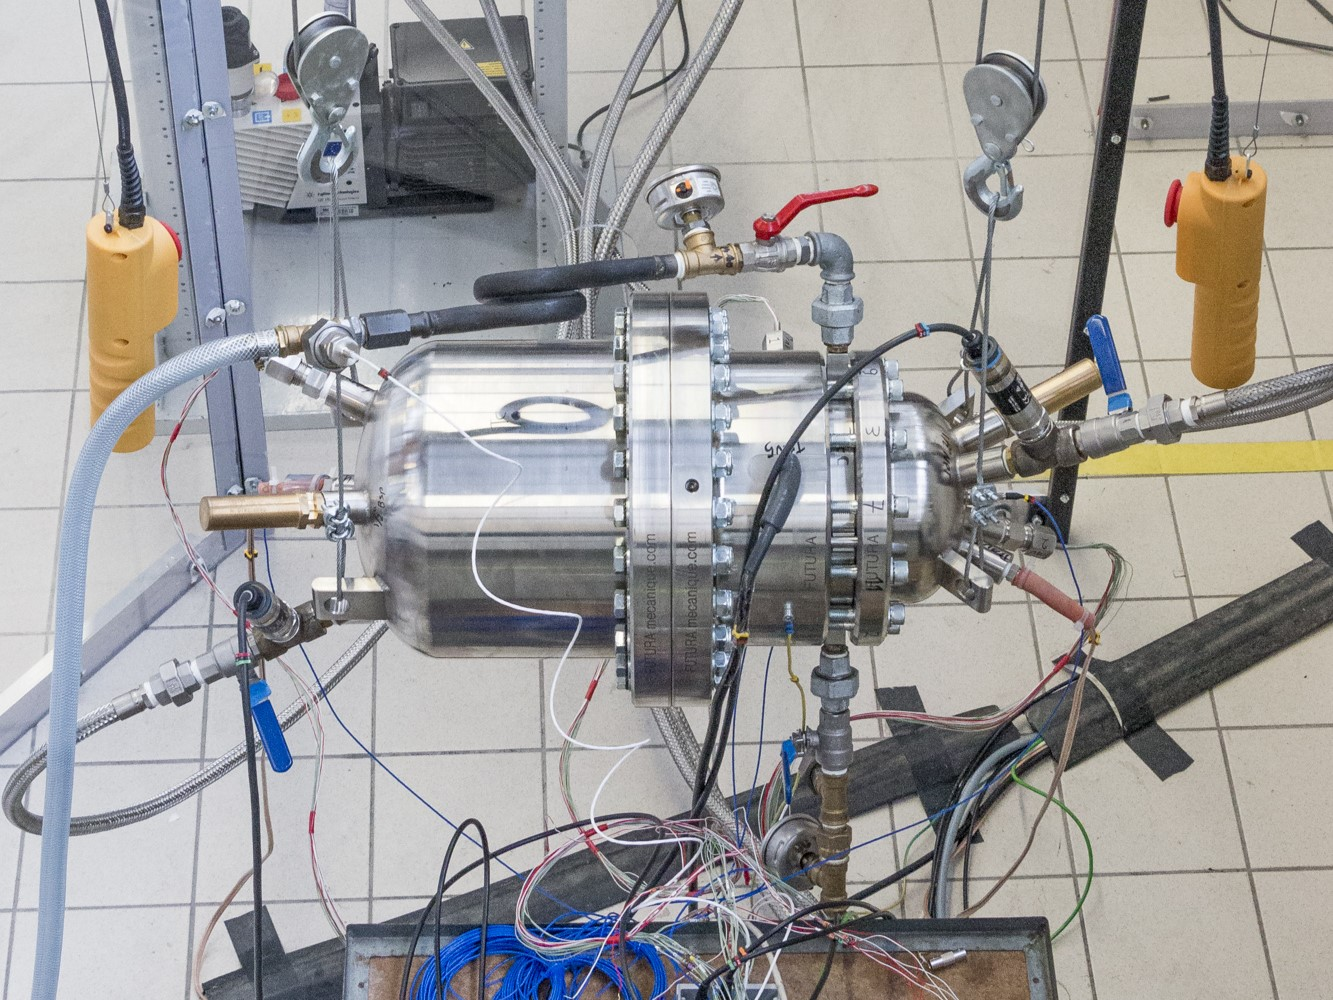
\includegraphics[width=\textwidth]{../fig/fig_SystemeAccroche/Machine_horizBetter_cropped.jpg}
		\caption{}
		\label{fig:TACOTSuspendu_Frigo}
	\end{subfigure}		%
	\begin{subfigure}{.47\textwidth}
		\centering
		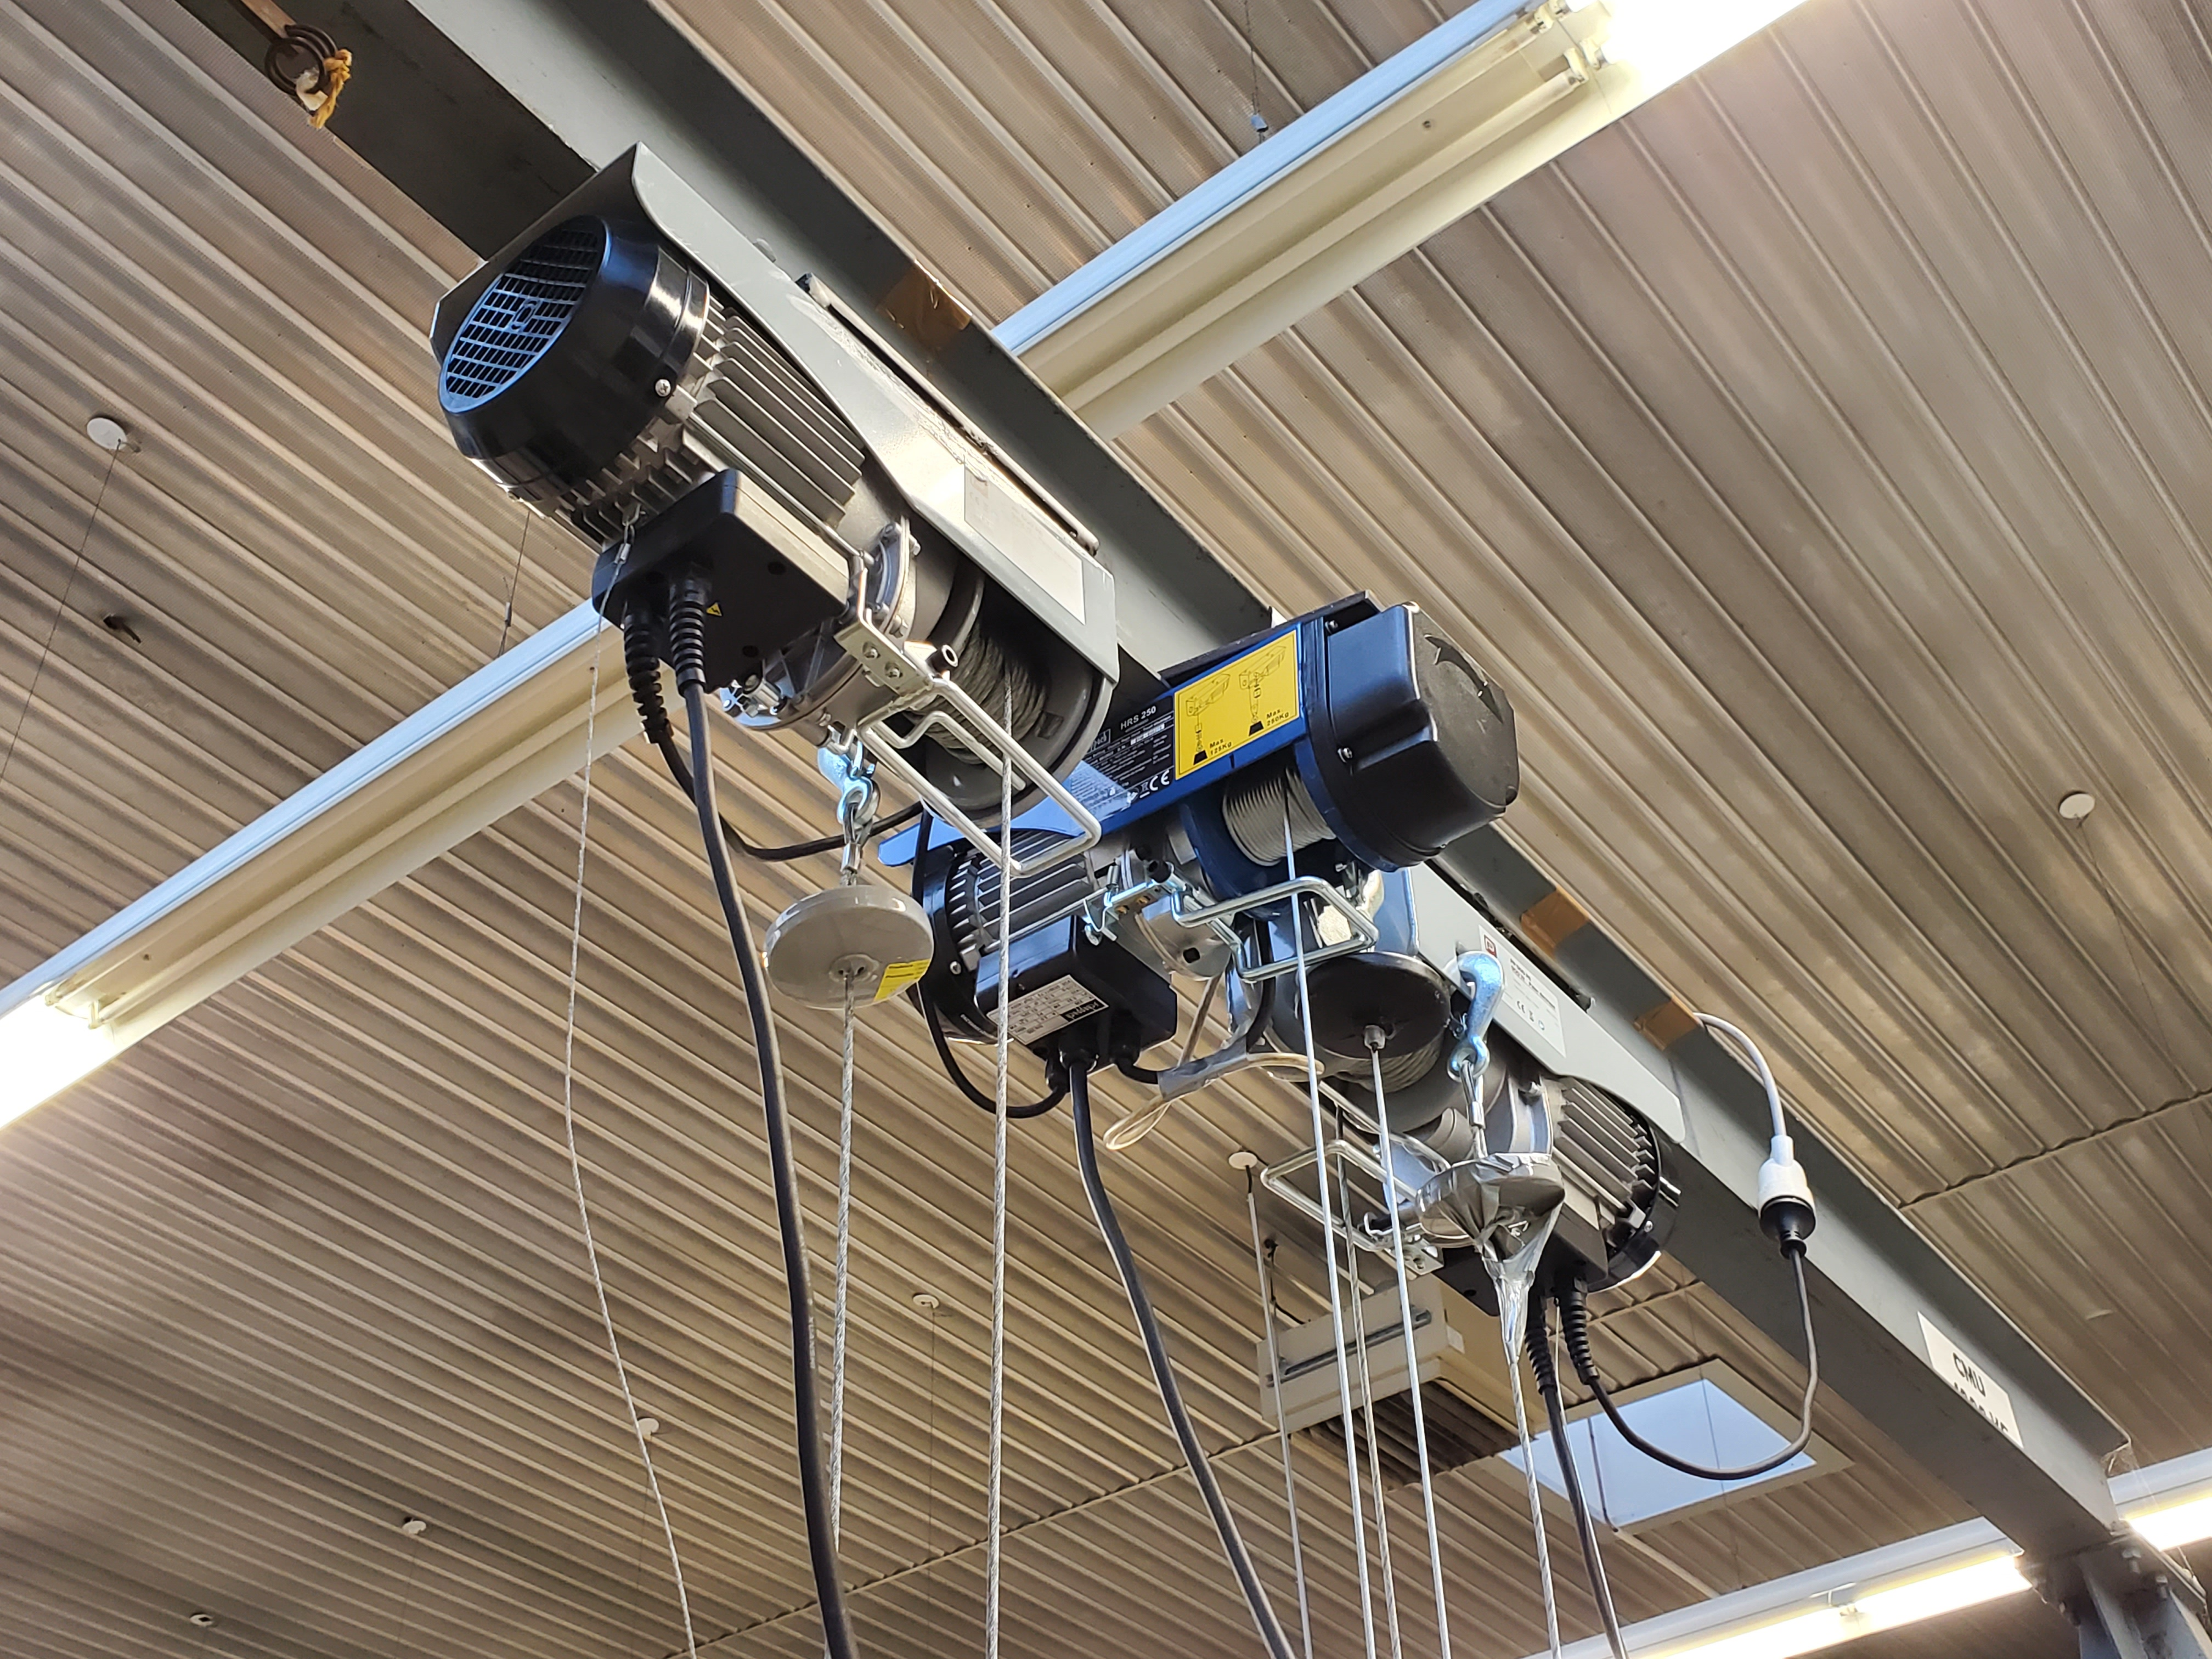
\includegraphics[width=\textwidth]{../fig/fig_SystemeAccroche/Palans.jpg}
		\caption{}
		\label{fig:TACOTSuspendu_Palans}
	\end{subfigure}	    
    \caption{Photographies \subref{fig:TACOTSuspendu_Frigo} du refrigérateur accroché et \subref{fig:TACOTSuspendu_Palans} des palans formant le système de suspension.}
    \label{fig:TACOTSuspendu}
\end{figure}

\subsection{Définition des orientations}

Les orientations choisies au moyen des palans sont décrites par deux angles $\psi_v$ et $\psi_h$. Le premier désigne l'angle entre l'axe horizontal et l'axe de symétrie du réfrigérateur, tandis que le second, la rotation autour de cet axe de symétrie. Les orientations utilisées dans les différentes parties de ce manuscript sont présentées sur la figure~\ref{fig:OrientationCore}. Cette figure, dans laquelle la gravité est toujours dirigée vers le bas de la page, présente également les emplacements des thermocouples utilisés. 

%\begin{figure}[!ht]
%    \centering
%    \external{fig_OrientationCore}
%%    \externalremake
%    \begin{tikzpicture}
%    \def\lenreg{2};
%    \def\diam{3};
    \def\spy{2};
    \def\xdist{8cm};
    \def\ydist{-7cm};
%    \def\persp{20};
%    
%    \def\LX{1};
%    \def\LY{2};
%    \def\CoreX{1.5};
%    \def\CoreY{.9*\LY};
%    

	\def\L{2};
	\def\R{6};
	\def\HX{.25};
	\def\decalage{\R/2-\L/2};
    
%	Islam's idea
	\begin{scope}
%		\begin{tikzpicture}[scale=2/3]

%    \def\lenreg{2};
%    \def\diam{3};
    \def\spy{2};
    \def\xdist{8cm};
    \def\ydist{-7cm};
%    \def\persp{20};
%    
%    \def\LX{1};
%    \def\LY{2};
%    \def\CoreX{1.5};
%    \def\CoreY{.9*\LY};
%    

	\def\L{2.1};
	\def\R{5};
	\def\HX{.25};
	\def\decalage{\R/2-\L/2};
	
		\draw(6.5,\R/2) node{\includegraphics[width=.8\textwidth]{../fig/fig_OrientationCore/tex/TACOT.png}};
			
		\fill[right color=blue!25,left color=red!25, draw=black] (\decalage,0) rectangle ++(\L,\R);
		\draw[fill=red!25] (\decalage,0) rectangle ++(-\HX,\R);
		\draw[fill=blue!25] (\decalage+\L,0) rectangle ++(\HX,\R);

		\foreach \z [evaluate=\z] in {0,...,4}{
			\foreach \r [evaluate=\r as \num using int(\r+1 + 3*\z)] in {0,...,2}{
				\draw ({\decalage+.5+\L-\z*(1+\L)/4},{-(\R-.4)/2*\r+\R-.2}) node[minimum size=10pt,draw,circle,fill=white,opacity=.7,text opacity=1]{} node(n\z\r){\scriptsize \num};
}}

%		\draw (n01.east) node [right]{0 $\rightarrow$ \begin{tabular}{l}Source\\acoustique\\principale\end{tabular}};
		\draw ($(n01)+(1.5,0)$) node[minimum size=10pt,draw,circle,fill=white,opacity=.7,text opacity=1]{} node(RIX) {\scriptsize 0};% node[anchor=west]{\begin{tabular}{rl}
%		& Source\\
%		$\rightarrow$ & acoustique\\
%		& principale
%		\end{tabular}};
		\draw (n30.north west) node [above, fill=white, fill opacity=.7, text opacity=1]{Ambiant};
		\draw (n10.north east) node [above, fill=white, fill opacity=.7, text opacity=1]{Froid};
\end{tikzpicture}
		\fill[right color=blue!25,left color=red!25, draw=black] (\decalage,0) rectangle ++(\L,\R);
		\draw[fill=red!25] (\decalage,0) rectangle ++(-\HX,\R);
		\draw[fill=blue!25] (\decalage+\L,0) rectangle ++(\HX,\R);

		\foreach \z [evaluate=\z] in {0,...,4}{
			\foreach \r [evaluate=\r as \num using int(\r+1 + 3*\z)] in {0,...,2}{
				\draw ({\decalage+.5+\L-\z*(1+\L)/4},{-(\R-.4)/2*\r+\R-.2}) node(n\z\r){\num};
}}

		\draw (n01.east) node [right]{$\rightarrow$ \begin{tabular}{l}Source\\acoustique\\principale\end{tabular}};
		\draw (n30.north west) node [above]{AHX};
		\draw (n10.north east) node [above]{CHX};

		\draw (0,\R+\spy) node [anchor=west]{\textbf{(a)} \texttt{H1}};

	\end{scope}
	
	
	
	\begin{scope}[xshift=\xdist-1cm,yshift=2cm]
		\begin{scope}[xslant=1,yscale=.5]
%		\begin{tikzpicture}[scale=2/3]

%    \def\lenreg{2};
%    \def\diam{3};
    \def\spy{2};
    \def\xdist{8cm};
    \def\ydist{-7cm};
%    \def\persp{20};
%    
%    \def\LX{1};
%    \def\LY{2};
%    \def\CoreX{1.5};
%    \def\CoreY{.9*\LY};
%    

	\def\L{1};
	\def\R{5};
	\def\HX{.25};
	\def\decalage{\R/2-\L/2};
	
%	\draw[opacity=0] (\decalage,0) rectangle ++(-\HX,\R); %%% Pour l'alignement vertical
%\draw{[white](\L/2,0) -- ++(0,\R);
	
	\begin{scope}[yslant=-1]
		\begin{scope}[xslant=.71]%, rotate=90, xscale=1]
		\node at (\decalage-\HX,0) (NewO) {};
%		\draw[->, very thick] (NewO.center) -- ++(0,1.2*\R);
%		\draw[->, very thick] (NewO.center) -- ++(1.2*\R,0);
		
		\fill[shading=axis,right color=MatlabBlue,left color=MatlabOrange, shading angle=22.5, draw=black] (\decalage,0) rectangle ++(\L,\R*1.4);
		\draw[fill=MatlabOrange] (\decalage,0) rectangle ++(-\HX,\R*1.4);
		\draw[fill=MatlabBlue] (\decalage+\L,0) rectangle ++(\HX,\R*1.4);

		\foreach \z [evaluate=\z] in {0,...,4}{
			\foreach \r [evaluate=\r as \num using int(\r+1 + 3*\z)] in {0,...,2}{
				\draw ({\decalage+.5+\L-\z*(1+\L)/4},{-(\R*1.4-.4)/2*\r+\R*1.4-.2}) node[minimum size=10pt,draw,circle,fill=white,opacity=.7,text opacity=1]{} node(n\z\r){\scriptsize \num};
}}

%		\draw (n01.east) node [right]{$\rightarrow$ \begin{tabular}{l}Source\\acoustique\\principale\end{tabular}};
		\draw ($(n01)+(.75,0)$) node[minimum size=10pt,draw,circle,fill=white,opacity=.7,text opacity=1]{} node {\scriptsize 0};% node[anchor=west]{\begin{tabular}{rl}
%		& Src\\
%		$\rightarrow$ & ac\\
%		& princ
%		\end{tabular}};
%		\draw (n30.north west) node [above right, fill=white, fill opacity=0, text opacity=1]{\textcolor{MatlabOrange}{\textbf{Ambiant}}};
%		\draw (n10.north east) node [above right, fill=white, fill opacity=0, text opacity=1]{\textcolor{MatlabBlue}{\textbf{Froid}}};
		
	\end{scope}
	\end{scope}
	\begin{pgfonlayer}{background}
		\draw[->, very thick] (NewO.center) -- ++(22.5:1.2*\R) node [above] {$\mathbf e_{y,0}$};
		\draw[->, very thick] (NewO.center) -- ++(90:1.2*\R) node [left] {$\mathbf e_{z,0}$};
		\draw[->, very thick] (NewO.center) -- ++(-45:1.2*\R) node [right] {$\mathbf e_{x,0}$};
  	\end{pgfonlayer}
\end{tikzpicture}
		\fill[right color=blue!25,left color=red!25, draw=black] (\decalage,0) rectangle ++(\L,\R);
		\draw[fill=red!25] (\decalage,0) rectangle ++(-\HX,\R);
		\draw[fill=blue!25] (\decalage+\L,0) rectangle ++(\HX,\R);

		\foreach \z [evaluate=\z] in {0,...,4}{
			\foreach \r [evaluate=\r as \num using int(\r+1 + 3*\z)] in {0,...,2}{
				\draw ({\decalage+.5+\L-\z*(1+\L)/4},{-(\R-.4)/2*\r+\R-.2}) node(n\z\r){\num};
}}

		\draw (n01.east) node [right]{$\rightarrow$ \begin{tabular}{l}Source\\acoustique\\principale\end{tabular}};
		\draw (n30.north west) node [above]{AHX};
		\draw (n10.north east) node [above]{CHX};
		\end{scope}

		\draw (1cm,\R+\spy-2cm) node [anchor=west]{\textbf{(b)} \texttt{H2}};
	\end{scope}  
	
	
	  
	\begin{scope}[yshift=\ydist]
%		%\fill[top color=red!25, bottom color=blue!25, draw=black] (0,0) rectangle ++(\R,\L);
%\draw[fill=blue!25] (0,0) rectangle ++(\R,-\HX);
%\draw[fill=red!25] (0,\L) rectangle ++(\R,\HX);
%
%\foreach \z [evaluate=\z] in {0,...,4}{
%	\foreach \r [evaluate=\r as \num using int(\r+1 + 3*\z)] in {0,...,2}{
%		\draw ({-(\R-.4)/2*\r+\R-.2},{\z*(1+\L)/4-.5}) node(n\z\r){\num};
%}}
%
%\draw (n40.south east) node [right]{AHX};
%\draw (n00.north east) node[right]{CHX};
%\draw (n01.south) node [below]{\shortstack{ $\downarrow$ \\Source acoustique principale}};
%
%\draw (0,\L+2*\HX+\spy) node [anchor=west]{\textbf{(c)} \texttt{V1}};

\begin{tikzpicture}[scale=2/3]

%    \def\lenreg{2};
%    \def\diam{3};
    \def\spy{2};
    \def\xdist{8cm};
    \def\ydist{-7cm};
%    \def\persp{20};
%    
%    \def\LX{1};
%    \def\LY{2};
%    \def\CoreX{1.5};
%    \def\CoreY{.9*\LY};
%    

	\def\L{2};
	\def\R{5};
	\def\HX{.35};
	\def\decalage{\R/2-\L/2};
	
	\begin{scope}[yslant=tan(22.5)]	
		
		\node at (0,-\HX) (NewO) {};
	
		\fill[shading=axis,right color=MatlabBlue,left color=MatlabOrange, shading angle=22.5, draw=black] (0,0) rectangle ++(\R,\L);
		\draw[fill=MatlabBlue] (0,0) rectangle ++(\R,-\HX);
		\draw[fill=MatlabOrange] (0,\L) rectangle ++(\R,\HX);

		\foreach \z [evaluate=\z] in {0,...,4}{
			\foreach \r [evaluate=\r as \num using int(\r+1 + 3*\z)] in {0,...,2}{
				\draw ({-(\R-.4)/2*\r+\R-.2},{\z*(1+\L)/4-.5}) node[minimum size=10pt,draw,circle,fill=white,opacity=.7,text opacity=1]{} node(n\z\r){\scriptsize \num};
}}

%		\draw (n40.south east) node [right, fill=white, fill opacity=0, text opacity=1]{\textcolor{MatlabOrange}{\textbf{Ambiant}}};
%		\draw (n00.north east) node[right, fill=white, fill opacity=0, text opacity=1]{\textcolor{MatlabBlue}{\textbf{Froid}}};
		\draw ($(n01.south)+(0,-1.1)$) node[minimum size=10pt,draw,circle,fill=white,opacity=.7,text opacity=1]{} node (RIX){\scriptsize 0};% node[anchor=north]{\begin{tabular}{c}
%		$\downarrow$\\
%		Source acoustique principale
%		\end{tabular}};

	\end{scope}
	\begin{pgfonlayer}{background}
		\draw[->, very thick] (NewO.center) -- ++(22.5:1.2*\R) node [above] {$\mathbf e_{y,0}$};
		\draw[->, very thick] (NewO.center) -- ++(90:1.2*\R) node [left] {$\mathbf e_{z,0}$};
		\draw[->, very thick] (NewO.center) -- ++(-45:1.2*\R) node [right] {$\mathbf e_{x,0}$};
  	\end{pgfonlayer}		
\end{tikzpicture}		

		\fill[top color=red!25, bottom color=blue!25, draw=black] (0,0) rectangle ++(\R,\L);
		\draw[fill=blue!25] (0,0) rectangle ++(\R,-\HX);
		\draw[fill=red!25] (0,\L) rectangle ++(\R,\HX);

		\foreach \z [evaluate=\z] in {0,...,4}{
			\foreach \r [evaluate=\r as \num using int(\r+1 + 3*\z)] in {0,...,2}{
				\draw ({-(\R-.4)/2*\r+\R-.2},{\z*(1+\L)/4-.5}) node(n\z\r){\num};
}}

		\draw (n40.south east) node [right]{AHX};
		\draw (n00.north east) node[right]{CHX};
		\draw (n01.south) node [below]{\shortstack{ $\downarrow$ \\Source acoustique principale}};

		\draw (0,\L+2*\HX+\spy) node [anchor=west]{\textbf{(c)} \texttt{V1}};
	\end{scope} 
	
	
	
	   
	\begin{scope}[xshift=\xdist,yshift=\ydist]
%		%\fill[top color=blue!25, bottom color=red!25, draw=black] (0,0) rectangle ++(\R,\L);
%\draw[fill=red!25] (0,0) rectangle ++(\R,-\HX);
%\draw[fill=blue!25] (0,\L) rectangle ++(\R,\HX);
%
%\foreach \z [evaluate=\z] in {0,...,4}{
%	\foreach \r [evaluate=\r as \num using int(\r+1 + 3*\z)] in {0,...,2}{
%		\draw ({(\R-.4)/2*\r+.2},{-\z*(1+\L)/4+\L+.5}) node(n\z\r){\num};
%}}
%
%\draw (n01.north) node [above]{\shortstack{Source acoustique principale\\ $\uparrow$}};
%\draw (n42.north east) node [right]{AHX};
%\draw (n02.south east) node [right]{CHX};
%
%\draw (0,\L+2*\HX+\spy) node [anchor=west]{\textbf{(d)} \texttt{V2}};

\begin{tikzpicture}[scale=2/3]

%    \def\lenreg{2};
%    \def\diam{3};
    \def\spy{2};
    \def\xdist{8cm};
    \def\ydist{-7cm};
%    \def\persp{20};
%    
%    \def\LX{1};
%    \def\LY{2};
%    \def\CoreX{1.5};
%    \def\CoreY{.9*\LY};
%    

	\def\L{2.1};
	\def\R{5};
	\def\HX{.25};
	\def\decalage{\R/2-\L/2};

		\fill[top color=MatlabBlue, bottom color=MatlabOrange, draw=black] (0,0) rectangle ++(\R,\L);
		\draw[fill=MatlabOrange] (0,0) rectangle ++(\R,-\HX);
		\draw[fill=MatlabBlue] (0,\L) rectangle ++(\R,\HX);

		\foreach \z [evaluate=\z] in {0,...,4}{
			\foreach \r [evaluate=\r as \num using int(\r+1 + 3*\z)] in {0,...,2}{
				\draw ({(\R-.4)/2*\r+.2},{-\z*(1+\L)/4+\L+.5}) node[minimum size=10pt,draw,circle,fill=white,opacity=.7,text opacity=1]{} node(n\z\r){\scriptsize \num};
}}

		\draw ($(n01.north)+(0,1.1)$) node[minimum size=10pt,draw,circle,fill=white,opacity=.7,text opacity=1]{} node(RIX){\scriptsize 0};% node[anchor=south]{\begin{tabular}{c}
%		Source acoustique principale\\
%		$\uparrow$
%		\end{tabular}};
		\draw (n42.north east) node [right, fill=white, fill opacity=.7, text opacity=1]{\textcolor{MatlabOrange}{\textbf{Ambiant}}};
		\draw (n02.south east) node [right, fill=white, fill opacity=.7, text opacity=1]{\textcolor{MatlabBlue}{\textbf{Froid}}};
%		\draw (n41.south) node [below]{\textcolor{white}{\shortstack{Source acoustique principale\\ $\uparrow$}}};
		
\end{tikzpicture}	
		\fill[top color=blue!25, bottom color=red!25, draw=black] (0,0) rectangle ++(\R,\L);
		\draw[fill=red!25] (0,0) rectangle ++(\R,-\HX);
		\draw[fill=blue!25] (0,\L) rectangle ++(\R,\HX);

		\foreach \z [evaluate=\z] in {0,...,4}{
			\foreach \r [evaluate=\r as \num using int(\r+1 + 3*\z)] in {0,...,2}{
				\draw ({(\R-.4)/2*\r+.2},{-\z*(1+\L)/4+\L+.5}) node(n\z\r){\num};
}}

		\draw (n01.north) node [above]{\shortstack{Source acoustique principale\\ $\uparrow$}};
		\draw (n42.north east) node [right]{AHX};
		\draw (n02.south east) node [right]{CHX};

		\draw (0,\L+2*\HX+\spy) node [anchor=west]{\textbf{(d)} \texttt{V2}};	
	\end{scope}    
    
%	 Alternate version    
%    \draw[->] (5.5,-.5) -- ++(1,0);\draw(6,-1) node[]{Vertical 2};
%    \draw[->] (6.5,.5) -- ++(-1,0);\draw(6,1) node[]{Vertical 1};
%    \draw[->] (9,.5) -- ++(0,-1);\draw(9,1) node[]{Horizontal 1};
%    \draw (12,0) node[circle,draw]{.};\draw (12,1) node[]{Horizontal 2};
%    
%    
%    \draw[line width=.5mm] (-2.5*\LX,0) to[out=90,in=-180] (-\LX,\LY) -- ++(2*\LX,0) -- ++(.5*\LX,-2*\LY/3) -- ++(.2*\LX,0) -- ++(0,2*\LY/3);
\draw[line width=.5mm] (\LX,\LY) -- ++(\LX,0) to[out=0,in=90] (3.5*\LX,0);

\fill[left color=red,right color=blue] ({-\LX+.4*\CoreX},0) rectangle ({-\LX+.9*\CoreX},\CoreY);
\draw[line width=.5mm] (-\LX,\CoreY) -- ++(\CoreX,0);
\draw[fill=PythonBlue] (-.9*\LX,0) -- ++(0,\CoreY) to[out=-80,in=90] (-.7*\LX,0);
\draw ({-\LX+.4*\CoreX},0) -- ++(0,\CoreY);
\draw ({-\LX+.9*\CoreX},0) -- ++(0,\CoreY);

\draw[fill=PythonBlue] (1.6*\LX,0) |- ++(.3*\LX,.9*\LY/3) |- ++(\LX,.2*\LY) arc (90:0:.05) -- ++(0,-.5*\LY);
%    \begin{scope}[yscale=-1]
%        \draw[line width=.5mm] (-2.5*\LX,0) to[out=90,in=-180] (-\LX,\LY) -- ++(2*\LX,0) -- ++(.5*\LX,-2*\LY/3) -- ++(.2*\LX,0) -- ++(0,2*\LY/3);
\draw[line width=.5mm] (\LX,\LY) -- ++(\LX,0) to[out=0,in=90] (3.5*\LX,0);

\fill[left color=red,right color=blue] ({-\LX+.4*\CoreX},0) rectangle ({-\LX+.9*\CoreX},\CoreY);
\draw[line width=.5mm] (-\LX,\CoreY) -- ++(\CoreX,0);
\draw[fill=PythonBlue] (-.9*\LX,0) -- ++(0,\CoreY) to[out=-80,in=90] (-.7*\LX,0);
\draw ({-\LX+.4*\CoreX},0) -- ++(0,\CoreY);
\draw ({-\LX+.9*\CoreX},0) -- ++(0,\CoreY);

\draw[fill=PythonBlue] (1.6*\LX,0) |- ++(.3*\LX,.9*\LY/3) |- ++(\LX,.2*\LY) arc (90:0:.05) -- ++(0,-.5*\LY);
%    \end{scope}
    
    % Old version
    % %%%%%%%%%%%%%%%%%%%% V1
    % \fill[bottom color=PythonBlue, top color=PythonRed,draw=black] (-\xdist,{\ydist+\lenreg}) -- ++(0,{-\lenreg}) arc (0:-180:{\diam} and {\diam/\persp}) -- ++(0,{\lenreg}) arc (-180:0:{\diam} and {\diam/\persp}) --cycle;
    
    % \draw[fill=PythonRed] ({-\xdist-\diam},\ydist+\lenreg) ellipse ({\diam} and {\diam/\persp});
    
    % \draw ({-\xdist-\diam},\ydist-\spy) node []{\textbf{(a)} V1};
    
    
    % %%%%%%%%%%%%%%%%%%%% V2
    % \fill[bottom color=PythonRed, top color=PythonBlue,draw=black] (\xdist,{\ydist+\lenreg}) -- ++(0,{-\lenreg}) arc (-180:0:{\diam} and {\diam/\persp}) -- ++(0,{\lenreg}) arc (0:-180:{\diam} and {\diam/\persp}) --cycle;
    
    % \draw[fill=PythonBlue] ({\xdist+\diam},\ydist+\lenreg) ellipse ({\diam} and {\diam/\persp});
    
    % \draw ({\xdist+\diam},\ydist-\spy) node []{\textbf{(b)} V2};
    
    
    % %%%%%%%%%%%%%%%%%%%% H1
    % \draw ({-\xdist-\diam},-\ydist) circle (\diam);
    % \draw[dashed,very thick] ({-\xdist-\diam},{-\ydist+\diam}) -- ++(0,-2*\diam);
    
    % \draw ({-\xdist-\diam},-\ydist-\diam-\spy) node []{\textbf{(c)} H1};
    
    
    % %%%%%%%%%%%%%%%%%%%% H2
    % \draw ({\xdist+\diam},-\ydist) circle (\diam);
    % \draw[dashed,very thick] ({\xdist},{-\ydist}) -- ++(2*\diam,0);
    
    % \draw ({\xdist+\diam},-\ydist-\diam-\spy) node []{\textbf{(d)} H2};
\end{tikzpicture}
%    \caption{Différentes orientations du c\oe{}ur thermoacoustique avec les positions des thermocouples et leurs numéro. Pour chaque cas, la gravité est orientée vers le bas. Les orientations correspondent aux angles {\bf (a)} $\psi_v=\ang{0}$ et $\psi_h=\ang{0}$ pour l'orientation `\texttt{H1}', {\bf (b)} $\psi_v=\ang{0}$ et $\psi_h=\ang{+90}$ pour l'orientation `\texttt{H2}', {\bf (c)} $\psi_v=\ang{-90}$ pour l'orientation `\texttt{V1}', et {\bf (d)} $\psi_v=\ang{+90}$ pour l'orientation `\texttt{V2}'.\textcolor{red}{CHX et AHX OK ou éch. froid et éch. chaud ? + $\psi_i$ dans la caption ou la figure ?}}
%    \label{fig:OrientationCore}
%\end{figure}

\begin{figure}[!ht]
    \centering
	\begin{subfigure}[c]{.47\textwidth}
		\centering
		\begin{tikzpicture}[scale=2/3]

%    \def\lenreg{2};
%    \def\diam{3};
    \def\spy{2};
    \def\xdist{8cm};
    \def\ydist{-7cm};
%    \def\persp{20};
%    
%    \def\LX{1};
%    \def\LY{2};
%    \def\CoreX{1.5};
%    \def\CoreY{.9*\LY};
%    

	\def\L{2.1};
	\def\R{5};
	\def\HX{.25};
	\def\decalage{\R/2-\L/2};
	
		\draw(6.5,\R/2) node{\includegraphics[width=.8\textwidth]{../fig/fig_OrientationCore/tex/TACOT.png}};
			
		\fill[right color=blue!25,left color=red!25, draw=black] (\decalage,0) rectangle ++(\L,\R);
		\draw[fill=red!25] (\decalage,0) rectangle ++(-\HX,\R);
		\draw[fill=blue!25] (\decalage+\L,0) rectangle ++(\HX,\R);

		\foreach \z [evaluate=\z] in {0,...,4}{
			\foreach \r [evaluate=\r as \num using int(\r+1 + 3*\z)] in {0,...,2}{
				\draw ({\decalage+.5+\L-\z*(1+\L)/4},{-(\R-.4)/2*\r+\R-.2}) node[minimum size=10pt,draw,circle,fill=white,opacity=.7,text opacity=1]{} node(n\z\r){\scriptsize \num};
}}

%		\draw (n01.east) node [right]{0 $\rightarrow$ \begin{tabular}{l}Source\\acoustique\\principale\end{tabular}};
		\draw ($(n01)+(1.5,0)$) node[minimum size=10pt,draw,circle,fill=white,opacity=.7,text opacity=1]{} node(RIX) {\scriptsize 0};% node[anchor=west]{\begin{tabular}{rl}
%		& Source\\
%		$\rightarrow$ & acoustique\\
%		& principale
%		\end{tabular}};
		\draw (n30.north west) node [above, fill=white, fill opacity=.7, text opacity=1]{Ambiant};
		\draw (n10.north east) node [above, fill=white, fill opacity=.7, text opacity=1]{Froid};
\end{tikzpicture}
		\caption{`\texttt{H1}'}
		\label{fig:OrientationCore_H1}
	\end{subfigure}		%
	\begin{subfigure}[c]{.47\textwidth}
		\centering
		\begin{tikzpicture}[scale=2/3]

%    \def\lenreg{2};
%    \def\diam{3};
    \def\spy{2};
    \def\xdist{8cm};
    \def\ydist{-7cm};
%    \def\persp{20};
%    
%    \def\LX{1};
%    \def\LY{2};
%    \def\CoreX{1.5};
%    \def\CoreY{.9*\LY};
%    

	\def\L{1};
	\def\R{5};
	\def\HX{.25};
	\def\decalage{\R/2-\L/2};
	
%	\draw[opacity=0] (\decalage,0) rectangle ++(-\HX,\R); %%% Pour l'alignement vertical
%\draw{[white](\L/2,0) -- ++(0,\R);
	
	\begin{scope}[yslant=-1]
		\begin{scope}[xslant=.71]%, rotate=90, xscale=1]
		\node at (\decalage-\HX,0) (NewO) {};
%		\draw[->, very thick] (NewO.center) -- ++(0,1.2*\R);
%		\draw[->, very thick] (NewO.center) -- ++(1.2*\R,0);
		
		\fill[shading=axis,right color=MatlabBlue,left color=MatlabOrange, shading angle=22.5, draw=black] (\decalage,0) rectangle ++(\L,\R*1.4);
		\draw[fill=MatlabOrange] (\decalage,0) rectangle ++(-\HX,\R*1.4);
		\draw[fill=MatlabBlue] (\decalage+\L,0) rectangle ++(\HX,\R*1.4);

		\foreach \z [evaluate=\z] in {0,...,4}{
			\foreach \r [evaluate=\r as \num using int(\r+1 + 3*\z)] in {0,...,2}{
				\draw ({\decalage+.5+\L-\z*(1+\L)/4},{-(\R*1.4-.4)/2*\r+\R*1.4-.2}) node[minimum size=10pt,draw,circle,fill=white,opacity=.7,text opacity=1]{} node(n\z\r){\scriptsize \num};
}}

%		\draw (n01.east) node [right]{$\rightarrow$ \begin{tabular}{l}Source\\acoustique\\principale\end{tabular}};
		\draw ($(n01)+(.75,0)$) node[minimum size=10pt,draw,circle,fill=white,opacity=.7,text opacity=1]{} node {\scriptsize 0};% node[anchor=west]{\begin{tabular}{rl}
%		& Src\\
%		$\rightarrow$ & ac\\
%		& princ
%		\end{tabular}};
%		\draw (n30.north west) node [above right, fill=white, fill opacity=0, text opacity=1]{\textcolor{MatlabOrange}{\textbf{Ambiant}}};
%		\draw (n10.north east) node [above right, fill=white, fill opacity=0, text opacity=1]{\textcolor{MatlabBlue}{\textbf{Froid}}};
		
	\end{scope}
	\end{scope}
	\begin{pgfonlayer}{background}
		\draw[->, very thick] (NewO.center) -- ++(22.5:1.2*\R) node [above] {$\mathbf e_{y,0}$};
		\draw[->, very thick] (NewO.center) -- ++(90:1.2*\R) node [left] {$\mathbf e_{z,0}$};
		\draw[->, very thick] (NewO.center) -- ++(-45:1.2*\R) node [right] {$\mathbf e_{x,0}$};
  	\end{pgfonlayer}
\end{tikzpicture}
		\caption{`\texttt{H2}'}
		\label{fig:OrientationCore_H2}
	\end{subfigure} \\ \vspace{1cm}
	\begin{subfigure}[c]{.47\textwidth}
		\centering
		%\fill[top color=red!25, bottom color=blue!25, draw=black] (0,0) rectangle ++(\R,\L);
%\draw[fill=blue!25] (0,0) rectangle ++(\R,-\HX);
%\draw[fill=red!25] (0,\L) rectangle ++(\R,\HX);
%
%\foreach \z [evaluate=\z] in {0,...,4}{
%	\foreach \r [evaluate=\r as \num using int(\r+1 + 3*\z)] in {0,...,2}{
%		\draw ({-(\R-.4)/2*\r+\R-.2},{\z*(1+\L)/4-.5}) node(n\z\r){\num};
%}}
%
%\draw (n40.south east) node [right]{AHX};
%\draw (n00.north east) node[right]{CHX};
%\draw (n01.south) node [below]{\shortstack{ $\downarrow$ \\Source acoustique principale}};
%
%\draw (0,\L+2*\HX+\spy) node [anchor=west]{\textbf{(c)} \texttt{V1}};

\begin{tikzpicture}[scale=2/3]

%    \def\lenreg{2};
%    \def\diam{3};
    \def\spy{2};
    \def\xdist{8cm};
    \def\ydist{-7cm};
%    \def\persp{20};
%    
%    \def\LX{1};
%    \def\LY{2};
%    \def\CoreX{1.5};
%    \def\CoreY{.9*\LY};
%    

	\def\L{2};
	\def\R{5};
	\def\HX{.35};
	\def\decalage{\R/2-\L/2};
	
	\begin{scope}[yslant=tan(22.5)]	
		
		\node at (0,-\HX) (NewO) {};
	
		\fill[shading=axis,right color=MatlabBlue,left color=MatlabOrange, shading angle=22.5, draw=black] (0,0) rectangle ++(\R,\L);
		\draw[fill=MatlabBlue] (0,0) rectangle ++(\R,-\HX);
		\draw[fill=MatlabOrange] (0,\L) rectangle ++(\R,\HX);

		\foreach \z [evaluate=\z] in {0,...,4}{
			\foreach \r [evaluate=\r as \num using int(\r+1 + 3*\z)] in {0,...,2}{
				\draw ({-(\R-.4)/2*\r+\R-.2},{\z*(1+\L)/4-.5}) node[minimum size=10pt,draw,circle,fill=white,opacity=.7,text opacity=1]{} node(n\z\r){\scriptsize \num};
}}

%		\draw (n40.south east) node [right, fill=white, fill opacity=0, text opacity=1]{\textcolor{MatlabOrange}{\textbf{Ambiant}}};
%		\draw (n00.north east) node[right, fill=white, fill opacity=0, text opacity=1]{\textcolor{MatlabBlue}{\textbf{Froid}}};
		\draw ($(n01.south)+(0,-1.1)$) node[minimum size=10pt,draw,circle,fill=white,opacity=.7,text opacity=1]{} node (RIX){\scriptsize 0};% node[anchor=north]{\begin{tabular}{c}
%		$\downarrow$\\
%		Source acoustique principale
%		\end{tabular}};

	\end{scope}
	\begin{pgfonlayer}{background}
		\draw[->, very thick] (NewO.center) -- ++(22.5:1.2*\R) node [above] {$\mathbf e_{y,0}$};
		\draw[->, very thick] (NewO.center) -- ++(90:1.2*\R) node [left] {$\mathbf e_{z,0}$};
		\draw[->, very thick] (NewO.center) -- ++(-45:1.2*\R) node [right] {$\mathbf e_{x,0}$};
  	\end{pgfonlayer}		
\end{tikzpicture}
		\caption{`\texttt{V1}'}
		\label{fig:OrientationCore_V1}
	\end{subfigure} %
	\begin{subfigure}[c]{.47\textwidth}
		\centering
		%\fill[top color=blue!25, bottom color=red!25, draw=black] (0,0) rectangle ++(\R,\L);
%\draw[fill=red!25] (0,0) rectangle ++(\R,-\HX);
%\draw[fill=blue!25] (0,\L) rectangle ++(\R,\HX);
%
%\foreach \z [evaluate=\z] in {0,...,4}{
%	\foreach \r [evaluate=\r as \num using int(\r+1 + 3*\z)] in {0,...,2}{
%		\draw ({(\R-.4)/2*\r+.2},{-\z*(1+\L)/4+\L+.5}) node(n\z\r){\num};
%}}
%
%\draw (n01.north) node [above]{\shortstack{Source acoustique principale\\ $\uparrow$}};
%\draw (n42.north east) node [right]{AHX};
%\draw (n02.south east) node [right]{CHX};
%
%\draw (0,\L+2*\HX+\spy) node [anchor=west]{\textbf{(d)} \texttt{V2}};

\begin{tikzpicture}[scale=2/3]

%    \def\lenreg{2};
%    \def\diam{3};
    \def\spy{2};
    \def\xdist{8cm};
    \def\ydist{-7cm};
%    \def\persp{20};
%    
%    \def\LX{1};
%    \def\LY{2};
%    \def\CoreX{1.5};
%    \def\CoreY{.9*\LY};
%    

	\def\L{2.1};
	\def\R{5};
	\def\HX{.25};
	\def\decalage{\R/2-\L/2};

		\fill[top color=MatlabBlue, bottom color=MatlabOrange, draw=black] (0,0) rectangle ++(\R,\L);
		\draw[fill=MatlabOrange] (0,0) rectangle ++(\R,-\HX);
		\draw[fill=MatlabBlue] (0,\L) rectangle ++(\R,\HX);

		\foreach \z [evaluate=\z] in {0,...,4}{
			\foreach \r [evaluate=\r as \num using int(\r+1 + 3*\z)] in {0,...,2}{
				\draw ({(\R-.4)/2*\r+.2},{-\z*(1+\L)/4+\L+.5}) node[minimum size=10pt,draw,circle,fill=white,opacity=.7,text opacity=1]{} node(n\z\r){\scriptsize \num};
}}

		\draw ($(n01.north)+(0,1.1)$) node[minimum size=10pt,draw,circle,fill=white,opacity=.7,text opacity=1]{} node(RIX){\scriptsize 0};% node[anchor=south]{\begin{tabular}{c}
%		Source acoustique principale\\
%		$\uparrow$
%		\end{tabular}};
		\draw (n42.north east) node [right, fill=white, fill opacity=.7, text opacity=1]{\textcolor{MatlabOrange}{\textbf{Ambiant}}};
		\draw (n02.south east) node [right, fill=white, fill opacity=.7, text opacity=1]{\textcolor{MatlabBlue}{\textbf{Froid}}};
%		\draw (n41.south) node [below]{\textcolor{white}{\shortstack{Source acoustique principale\\ $\uparrow$}}};
		
\end{tikzpicture}
		\caption{`\texttt{V2}'}
		\label{fig:OrientationCore_V2}
	\end{subfigure}   
    \caption{Différentes orientations du c\oe{}ur thermoacoustique avec les positions des thermocouples et leurs numéro. Pour chaque cas, la gravité est orientée vers le bas. Les orientations correspondent aux angles \subref{fig:OrientationCore_H1} $\psi_v=\ang{0}$ et $\psi_h=\ang{0}$ pour l'orientation `\texttt{H1}', \subref{fig:OrientationCore_H2} $\psi_v=\ang{0}$ et $\psi_h=\ang{+90}$ pour l'orientation `\texttt{H2}', \subref{fig:OrientationCore_V1} $\psi_v=\ang{-90}$ pour l'orientation `\texttt{V1}', et \subref{fig:OrientationCore_V2} $\psi_v=\ang{+90}$ pour l'orientation `\texttt{V2}'.}%\textcolor{red}{CHX et AHX OK ou éch. froid et éch. chaud ? + $\psi_i$ dans la caption ou la figure ?}}
    \label{fig:OrientationCore} %
\end{figure}

\medskip

La première orientation, nommée `\texttt{H1}' et représentée sur la figure~\ref{fig:OrientationCore_H1}, est la même que dans l'article dédié à la conception du réfrigérateur \cite{ramadan_design_2021}. Dans cette configuration, le \textsc{Tacot} est placé à l'horizontale comme sur la figure~\ref{fig:TACOTSuspendu_Frigo}, et les thermocouples sont placés sur un plan vertical coplanaire à la gravité. Cette orientation fait office de référence des orientations, soit $\psi_v=\psi_h=\qty{0}{\degree}$. \smallskip

Ensuite, la deuxième orientation est représentée sur la figure~\ref{fig:OrientationCore_H2}. Dans ce cas, référérencé en tant que `\texttt{H2}', le réfrigérateur est toujours à l'horizontale ($\psi_v=\qty{0}{\degree}$), mais pivoté autour de son axe pour placer les thermocouples sur un plan horizontal auquel la gravité est orthogonale ($\psi_h=\qty{90}{\degree}$).\medskip

L'orientation `\texttt{V1}' est affichée sur la figure~\ref{fig:OrientationCore_V1}. Cette configuration est radicalement différentes des deux précédentes : l'axe de symétrie du réfrigérateur est vertical, avec l'échangeur froid sous l'échangeur ambiant ($\psi_v=\qty{-90}{\degree}$). \smallskip

Enfin, l'orientation `\texttt{V2}' affichée sur la figure~\ref{fig:OrientationCore_V2} est l'orientation inverse de la précédente. L'axe de symétrie du réfrigérateur est encore vertical, mais la source acoustique principale est cette fois au dessus du noyau thermoacoustique et $\psi_v=\qty{+90}{\degree}$.

\subsection{Acquisitions}
\subsubsection{Procédures d'acquisition}
Les acquisitions sont réalisées en plusieurs temps. Tout d'abord et pour toutes les expériences,  l'état initial de toutes les grandeurs est acquis sur une minute et sauvegardé sous un label `\texttt{init}' à chaque début de journée de campagne. Cela permet de garder en mémoire toutes les conditions expérimentales initiales dont les valeurs peuvent potentiellement influer sur le comportement du réfrigérateur, comme par exemple la température ambiante ou la pression statique. \medskip

Ensuite, en prévision de la mesure de flux de chaleur $\dot Q_a$ extrait par l'échangeur ambiant (voir l'annexe~\ref{chap:AHX}), l'eau est préalablement mise en circulation dans cet échangeur après avoir démarré une acquisition des 30 capteurs jusqu'à stabilisation de la distribution de température dans le noyau. L'acquisition est ensuite interrompue et enregistrée avec un label `\texttt{Water}'. \bigskip

L'étape suivante dépend du type d'expérience menée : les mesures peuvent être sans ou avec acoustique, et ce, pour  différentes amplitudes de pression oscillante. En revanche, certains des paramètres d'excitation reste constant pour toutes les expériences :  le gaz est également le même dans toutes les expériences. Il est composé de \qty{65}{\percent} d'hélium et de \qty{35}{\percent} d'argon, et le tout est pressurisé à \qty{4e6}{\pascal}. Dans le cas des expériences à \textit{drive ratio} non nul, la fréquence est toujours de \qty{47}{\hertz}, car la prédiction des performances annonce les meilleurs résultats. C'est également la première fréquence de résonance de la source principale, et son facteur de qualité très élevé (\echaf{$Q_{ts}=$}) ainsi que la faible valeur de résistance de la bobine ($R_e=\qty{.7}{\ohm}$) empêchent l'amplificateur QSC de fonctionner à une autre fréquence sans l'endommager, l'impédance minimale supportée étant de \qty{2}{\ohm}. Ensuite, le déphasage inter-source $\varphi_{2-1}$ est également fixé à \ang{-60}, ce que le modèle \textsc{DeltaEC} indique comme déphasage optimale et que des expériences préliminaires confirment.

\paragraph{Mesures sans acoustique}\label{chap:MesureSansAcou}
Pour ces mesures de type `\texttt{heat\_{}only}', la charge thermique est appliquée au noyau sans alimenter les sources acoustiques. Cette charge thermique consiste en l'alimentation des cartouches chauffantes contenues dans l'échangeur froid par une puissance électrique connue, tandis qu'un débit d'eau de \qty{7}{\litre\per\minute} s'écoule dans l'échangeur ambiant qui se trouve de l'autre côté du noyau. 

Ces mesures \echaf{doivent} permettre d'étudier la distribution de température en l'absence d'écoulement oscillant, ainsi que de calculer les valeurs de conductivité thermique $k_x$ et $k_r$ ou les coefficients de pertes latérales $h_x$ et $h_r$.\medskip

Dans ce type d'expériences, les noms des zones \og froide \fg{} et \og ambiante \fg{} sont conservés pour des raisons de clarté, mais l'eau circulant dans l'échangeur ambiant et les cartouches chauffantes se trouvant dans l'échangeur froid, la direction du gradient de température dans le noyau thermoacoustique est inversée par rapport aux expériences avec acoustique. %Toutefois, les ordres de grandeur des différences de température sont les mêmes que pour les expériences avec acoustique, c'est-à-dire 

Pour garder un moyen de comparaison avec les mesures avec acoustique, le mélange de gaz est le même.

\paragraph{Mesures avec acoustique}\label{chap:MesureAvecAcou} 
Une acquisition étiquetée `\texttt{Acou}' est démarrée, puis les sources sont alimentées jusqu'à l'amplitude souhaitée. Au bout d'une heure, l'acquisition est arrêtée et sauvegardée. En l'absence d'expérience avec charge thermique, c'est la fin de l'expérience : toutes les sources acoustiques et circulations d'eau sont progressivement arrêtées et le réfrigérateur est laissé pour un retour à l'état initial.

Au cours de cette étude, trois amplitudes acoustiques sont choisies. La première correspond à un \textit{drive ratio} $DR=\frac{p}{P_0}=\qty{.4}{\percent}$, soit une amplitude très faible où l'effet thermoacoustique est à peine visible. Ainsi, l'hypothèse concernant la linéarité acoustique est mieux vérifiée et peut \textit{a priori} être plus aisément comparé à la théorie linéaire. À l'inverse, le \textit{drive ratio} de la deuxième amplitude est le plus élevé avec $DR=\qty{3.5}{\percent}$, et est celui pour lequel les performances du réfrigérateur ($COP$, $Q_f$, ...) sont les plus élevées obtenues avec cette machine \cite{ramadan_design_2021}, mais aussi qui présentent de forts écarts à la théorie. La troisième est choisie à un \textit{drive ratio} intermédiaire où $DR=\qty{2}{\percent}$. 




\subsubsection{Paramètres d'acquisition}
Comme dit précédemment, la fréquence de fonctionnement du \textsc{Tacot} est de \qty{47}{\hertz}, ce qui implique une fréquence d'échantillonnage au moins deux fois supérieure. Cependant, les cartes d'acquisition sont rassemblées sur une baie d'instrumentation, contraignent la fréquence d'échantillonage utilisée. Celles concernant les mesures de quantité oscillantes (pression acoustique, accélération \echaf{à vérifier}) imposent que la fréquence d'échantillonage $f_s$ soit au moins égale à \qty{1651}{\Hz}\footnote{Les acquisitions des \num{30} capteurs durent \qty{1}{\hour}, et les données sont encodées sur \qty{32}{\bit} flottants. Au total, chaque acquisition pèse \qty{713}{\mega\byte}, taille à laquelle il faut ajouter quelques \unit{\mega\byte} pour le protocole \texttt{tdms} et l'entête contenant les informations de mesure.}.

\section{Ensemble des simulations réalisées}\label{chap:SimusRealisees}
\subsection{Estimation théorique du flux de chaleur de convection naturelle}
Au sein du réfrigérateur \textsc{Tacot} et particulièrement dans la cavité devant la source acoustique principale, la distribution de température du côté froid hors du noyau laisse penser à la présence d'une cellule de convection naturelle à l'intérieur. Il est difficile de se rendre compte des flux massique et thermique causés par la différence de température de part et d'autre des différentes zones du \textsc{Tacot} -- Volume d'adaptation d'impédance, noyau thermoacoustique -- à cause de leurs géometries, du type de convection naturelle rencontré, de la porosité, etc. Des études hydrodynamiques sont menées pour aider à l'interprétation des mesures de température. \medskip

Tout d'abord, deux étude très simplifiées sont réalisées pour une cavité 2D différentiellement chauffée par des températures chaude $T_c$ et froide $T_f$. Cette étude doit permettre l'obtention d'ordres de grandeurs des quantité d'intérêt, en particulier le flux de chaleur $Q_{conv}$ qui agit comme une charge thermique sur le côté froid du noyau thermoacoustique. \smallskip

Ensuite, une simulation par éléments finis de cette cavité sur le logiciel Comsol Multiphysics doit permettre d'estimer les lignes de courants dans la cellule et l'influence de cet écoulement sur la distribution de température sur l'échangeur froid.

\subsubsection{\'Etude simplifiée}
\paragraph{Sans acoustique}
Pour introduire des concepts utiles à la compréhension des phénomènes de convection naturelle, une étude très simplifiée dans une cavité rectangulaire en 2D et représentée sur les figures~\ref{fig:SimuConvNat2D}\textbf{(a)} et \textbf{(b)} est menée. 

Dans la première sous-figure~\ref{fig:SimuConvNat2D}\textbf{(a)}, les parois verticales droite et gauche sont respectivement maintenues à une température froide $T_f$ et chaude $T_c$, tandis que le sol, le plafond et le gaz au repos sont à la température $T_\infty$. En régime stationnaire, il s'établit une cellule de convection naturelle dans laquelle le gaz est mis en mouvement par les  variations de masse volumique proches des parois verticales. Cette configuration s'apparente aux orientations `\texttt{H1}' et `\texttt{H2}', respectivement présentées sur les figures~\ref{fig:OrientationCore_H1} et \subref{fig:OrientationCore_H2}.

Dans la seconde sous-figure~\ref{fig:SimuConvNat2D}\textbf{(b)}, ce sont cette fois les sol et plafond qui sont fixés aux températures chaude $T_c$ et froide $T_f$, et les murs et le gaz au repos pour lesquels la température est $T_\infty$. Dans cette configuration, favorable a priori à la mise en place d'une instabilité de \og Rayleigh-Bénard \fg{}, il peut s'établir une ou plusieurs cellules de convection naturelle si le nombre de Rayleigh $\Rayleigh$ est supérieur à un nombre de Rayleigh critique $\Rayleigh_c$ \echaf{valeur 1700 ? + citation}. Le gaz s'élève de la paroi chaude jusqu'à la paroi froide, de laquelle il redescend ensuite pour revenir à son point de départ. Dans ce cas, la cellule de convection naturelle peut adopter une structure très complexe, plus que ce que peut suggérer la figure~\ref{fig:SimuConvNat2D}\textbf{(b)} qui ne représente qu'une illustration grossière du mouvement du fluide. Les expériences correspondant à ce cas sont mises en place en suivant les orientations `\texttt{V1}' et `\texttt{V2}', présentés respectivement sur les figures~\ref{fig:OrientationCore_V1} et \subref{fig:OrientationCore_V2}

\begin{figure}[!ht]
    \centering
    \external{fig_SimuConvNat2D}
%    \externalremake
    \begin{tikzpicture}[scale=.95]
	\def\l{5};
	\def\L{7};
	\def\e{.25};
	\def\xdist{9cm};
	\def\ylab{-.75};
		
	% ----------- Flow direction
	\draw[->,dashed,gray,very thick] (-\L/2.5,.5+\l/2) to[out=90,in=90] (\L/2.5,\l/2);
	\draw[->,dashed,gray,very thick] (\L/2.5,-.5+\l/2) to[out=-90,in=-90] (-\L/2.5,\l/2);
	
	% ----------- Rayleigh zone
%	\fill[dotted] (O.center) to[out=0,in=-90] ++(\e)
	
	% ----------- Cavity
	\fill[pattern=north east lines,pattern color=MatlabOrange] (-\L/2,\l) node[above left,color=MatlabOrange]{$T_{c}$} rectangle ++(-\e,-\l);
	\fill[pattern=north east lines,pattern color=MatlabBlue] (\L/2,\l) node[above right,color=MatlabBlue]{$T_{f}$} rectangle ++(\e,-\l);
	\draw[ultra thick] (-\L/2,0) rectangle ++(\L,\l);
	\draw (-\L/4,0) node(O)[above]{$T_{\infty}$};
	
	% ----------- Gravity direction	
	\draw[->,green!50!black] (0,2*\l/3) -- ++(0,-\l/3) node[midway,fill=white]{$\mathbf g$};
	
%	\draw[<->] (-\L/2,\l+.2) -- ++(\L,0) node[midway,above]{$L_c^{(1)}$};	
	
	
	\draw (0,\ylab) node[]{\textbf{(a)}};
	
	% ----------- Zoom sur paroi chaude
	\begin{scope}[xshift=\xdist]
%		\fill[dashed,left color=MatlabOrange!50,right color=white] (0,0) to[out=0,in=-90] node[near start,below right]{$T_\infty$} ++(2,\l) -| (0,0);
%		\draw[<->] (0.1,3*\l/4) -- ++(1.8,0) node[midway,below]{$L_c^{(1)}$};
%		\draw[dotted] (0,3*\l/4) to[out=45,in=135] node(v)[near end]{} ++(2,0) ;
%		\draw[dotted,->] ($(v.north east)+(.75,.5)$) node[right]{\shortstack{Profil\\de vitesse}} to[out=180,in=45] (v.north east) ;
%		\fill[pattern=north east lines,pattern color=MatlabOrange] (0,\l) node[above left,color=MatlabOrange]{$T_{c}$} rectangle ++(-\e,-\l);
%		\draw[ultra thick] (0,0) -- ++(0,\l);
%		
%		
		% ----------- Flow direction
		\foreach \xi in {1,2,3}{
		\node (bottom\xi) at ({\xi*\L/3-\L/6-\L/2},\l/8){};
		\node (top\xi) at ({\xi*\L/3-\L/6-\L/2},{7*\l/8}){};
		\draw[->,dashed,gray,very thick] (bottom\xi.north west) to[out=110,in=-110] (top\xi.south west);
		\draw[->,dashed,gray,very thick] (top\xi.south east) to[out=-70,in=70] (bottom\xi.north east);
		}
		
		% ----------- Cavity
		\fill[pattern=north east lines,pattern color=MatlabOrange] (-\L/2,0) rectangle ++(\L,-\e) node[right,color=MatlabOrange]{$T_{c}$};
		\fill[pattern=north east lines,pattern color=MatlabBlue] (-\L/2,\l) rectangle ++(\L,+\e) node[right,color=MatlabBlue]{$T_{f}$};
		\draw[ultra thick] (-\L/2,0) rectangle ++(\L,\l);% node(O2)[below left]{$T_{\infty}$};
		\draw (\L/2,3*\l/4) node[left]{$T_{\infty}$};
		
		% ----------- Gravity direction
		\draw[->,green!50!black] (0,2*\l/3) -- ++(0,-\l/3) node[midway,fill=white]{$\mathbf g$};
	
%		\draw[<->] (-\L/2-.2,0) -- ++(0,\l) node[midway,left]{$L_c^{(2)}$};	

		\draw (0,\ylab) node[]{\textbf{(b)}};
		
		
	\end{scope} 
	
		\draw[<->,dashed] (\xdist/2,0) -- ++(0,\l) node[midway,fill=white]{$L_c$};	
		\draw[gray,loosely dashed] (\L/2,0) -- (\xdist-\L/2,0) (\L/2,\l) -- (\xdist-\L/2,\l);
	
\end{tikzpicture}
    \caption{Cellule de convection naturelle dans une cavité rectangulaire 2D \textbf{(a)} pour un gradient de température normal à la direction de la gravité, et \textbf{(b)} pour un gradient de température colinéaire à la direction de la gravité. Cela dit, la distance caractéristique est \echaf{choisie} dans les deux cas suivant la même direction que la gravité.}
    \label{fig:SimuConvNat2D}
\end{figure}



Pour un tel système, il est possible de modéliser l'écoulement en utilisant les équations de Navier-Stokes, réécrites dans le système d'équations~\eqref{eq:NavierStokes_Boussinesq} avec l'approximation de Boussinesq tel que

\begin{subequations}
	\begin{align}
		\partial_t \delta\rho + (\mathbf v \cdot \nabla)\mathbf{\delta\rho} + \delta\rho \nabla \cdot \mathbf{v} &= 0, \label{eq:NavierStokes_Boussinesq_Conti}\\
		\delta\rho [\partial_t \mathbf v + (\mathbf v \cdot \nabla)\mathbf v] &= -\nabla p + \mu \nabla^2 \mathbf v + \delta\rho \mathbf g, \text{et}\label{eq:NavierStokes_Boussinesq_QtMvt}\\
		\partial_t T + (\mathbf v \cdot \nabla) T - \kappa\nabla^2T &= 0. \label{eq:NavierStokes_Boussinesq_NRJinterne}
	\end{align}
	\label{eq:NavierStokes_Boussinesq}%
\end{subequations}
La dédimensionalisation de l'équation \eqref{eq:NavierStokes_Boussinesq_QtMvt} qui concerne la conservation de la quantité de mouvement s'écrit

\begin{equation}
	\frac{1}{\mathrm{Pr}}(\partial_t \mathbf{v} + (\mathbf{v} \cdot \nabla)\mathbf{v}) = -\nabla p + \mathrm{Ra} T \mathbf e_z + \nabla^2 \cdot \mathbf{v},
	\label{eq:NonDim_NavierStokes_Boussinesq_QtMvt}
\end{equation}
et fait apparaître le nombre de Prandtl noté $\mathrm{Pr}$ déjà présenté dans l'équation \eqref{eq:Prandtl}, ainsi que le nombre de Rayleigh noté $\mathrm{Ra}$, et dont la définition est donnée par 
\begin{equation}
	\mathrm{Ra} = \frac{g \beta L_c^3}{\nu \kappa} (T_c-T_f),
	\label{eq:NbrRayleigh}
\end{equation}
où $T_c$ et $T_f$ sont les températures chaude et froide de part et d'autre de la zone considérée, et $L_c$ est la dimension caractéristique de la cavité suivant la direction verticale. Ce nombre est primordial car il correspond au rapport des effets gravifiques qui mettent le fluide en mouvement aux effets qui le limitent, soit la diffusion thermique qui limite la différence de température et la viscosité qui ralentit l'écoulement du fluide. Sa valeur indique également le régime de l'écoulement causé par la convection car des vitesses de référence verticales et horizontales, notées $v_{ref}^{// \mathbf g}$ et $v_{ref}^{\perp \mathbf g}$, peuvent d'ailleurs être calculées en fonction de ce nombre de Rayleigh suivant les définitions

\begin{subequations}
	\begin{align}
		v_{\sf ref}^{// \mathbf g} &\sim \frac{\kappa}{L_c}\sqrt{\Rayleigh} \text{ et}	\label{eq:VitesseReferenceV_Rayleigh}\\
		v_{\sf ref}^{\perp \mathbf g} &\sim \frac{\kappa}{L_c}\sqrt[4]{\Rayleigh},	\label{eq:VitesseReferenceH_Rayleigh}
	\end{align}
	\label{eq:VitesseReference_Rayleigh}%
\end{subequations}
d'après la réécriture en 2D des équations de conservation de la quantité de mouvement et de l'énergie par Belleoud et dans le cas où le gradient de température est lui-même horizontal \cite{belleoud_etude_2016}. \echaf{gradient vertical et Rayleigh critique pour apparition/stabilité de la cellule de Rayleigh-Bénard.}

Dans un matériau poreux, il peut également exister des écoulements liés à la convection naturelle. Dans ce cas, le nombre de Rayleigh est toujours une notion utile pour prédire le mouvement du fluide à l'intérieur, à condition toutefois de le modifier pour prendre en compte la perméabilité $K_p$ ainsi que la diffusivité thermique $\kappa_p$ de ce milieu. Il vient alors l'expression du nombre de Rayleigh-Darcy noté $\mathrm{Ra}_p$, et dont la définition est donnée par Nield et Bejan \cite{nield_convection_2013} par

\begin{equation}
	\mathrm{Ra}_p = \frac{g \beta L_c K_p}{\nu \kappa_p} (T_c-T_f),
	\label{eq:NbrRayleigh_poreux}
\end{equation}
ainsi que la vitesse verticale de référence correspondante, 

\begin{equation}
	v_{\textsf{ref},p}^{// \mathbf g} = \frac{\kappa_p}{L_c} \Rayleigh_p.
	\label{eq:VitesseReference_Rayleigh_poreux}
\end{equation}


Lorsque la convection naturelle provoque un écoulement circulant à une vitesse de référence $v_{\sf ref}$, il est possible de quantifier la contribution des échanges thermiques ainsi \echaf{provoqués/favorisés} et des pertes visqueuses en définissant le nombre de Grashof par

\begin{equation}
	\Grashof = \left( \frac{v_{\sf ref} L_c}{\nu} \right)^2,
	\label{eq:NbrGrashof}
\end{equation}
et qui est relié au nombre de Rayleigh par la formule

\begin{equation}
	\Grashof = \frac{\Rayleigh}{\Prandtl}.
	\label{eq:NbrGrashof_RayleighSurPrandtl}
\end{equation}


\paragraph{Avec acoustique}
Les termes précédents sont issus de la littérature en l'absence d'écoulement oscillant. Cette hypothèse n'a pas de sens dans le cas des expériences menées avec acoustique, et un autre indicateur est introduit pour quantifier les échanges de chaleur causé par un fluide en mouvement. Cet indicateur est le nombre de Péclet, noté $\Peclet$, et défini par

\begin{equation}
	\Peclet = \frac{v L_c}{\kappa}.
	\label{eq:NbrPeclet}
\end{equation}

Contrairement au nombre de Rayleigh qui sert à comparer le mouvement d'un fluide causé par un échange thermique, le nombre de Péclet quantifie les échanges de chaleur réalisés par un fluide qui se déplace. Cependant, il reste nécessaire de proposer une hypothèse quant à l'utilisation de ce nombre : la vitesse d'entraînement du fluide est ici la vitesse acoustique $v$, contrairement aux cas classiques de son utilisation dans la littérature où un écoulement continu est considéré. De même que le nombre de Rayleigh, le nombre de Péclet est lié aux nombres de Grashof et Prandtl suivant la relation 

\begin{equation}
	\Peclet \equiv \sqrt{\Grashof}~\Prandtl,
	\label{eq:NbrPeclet_GrashofFoisPrandtl}
\end{equation}
différente de l'équation~\eqref{eq:NbrGrashof_RayleighSurPrandtl}.

Ces échanges thermiques par convection sont à comparer aux transferts de chaleur par conduction. La prépondérance de chaque effet est donnée par le calcul du nombre de Nusselt, dont la définition est

\begin{equation}
	\Nusselt = \frac{h L_c}{k},
\end{equation}
avec $h$ le coefficient d'échange convectif.\bigskip

Les calculs des nombres précédent peuvent guider l'intuition quant aux prédominances de chaque effet prennant place dans le noyau et aux environs de celui-ci : la vitesse d'entraînement du gaz par convection, la quantité de chaleur transportée par elle, son importance par rapport à la conduction par le matériau poreux et ses parois.

\subsubsection{\'Elements finis}
\paragraph{Volume d'adaptation d'impédance}
Le modèle 2D simplifié ne prend pas en compte plusieurs paramètres : la cavité est en réalité un cône. Pour connaître l'allure des lignes de courant à l'intérieur en présence d'un flux de masse provoqué par la convection naturelle, un modèle de la cavité est réalisé dans le logiciel d'éléments finis Comsol Multiphysics grâce à une géométrie présenté sur la figure~\ref{fig:CaviteConvNat_ComsolGeometrie}. Avec ce logiciel, il est également possible de coupler une simulation acoustique en plus de la simulation de transferts thermiques, ce que le modèle 2D simplifié ne permet pas aisément.

\begin{figure}[!ht]
    \centering
    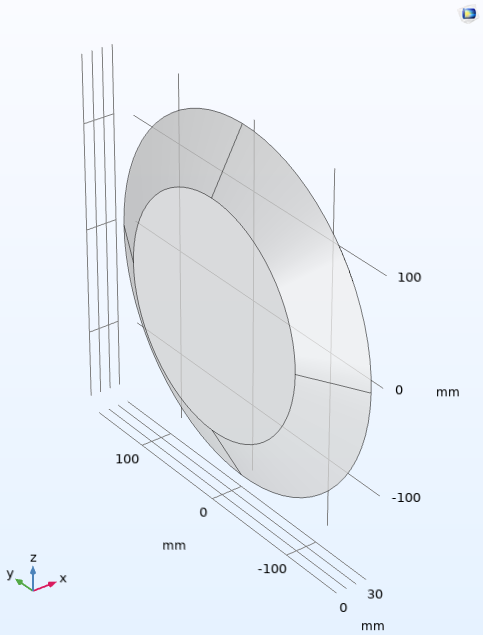
\includegraphics[width=.5\textwidth]{../fig/fig_ConvNatComsol/Geometry.png}
    \caption{Géométrie du volume d'adaptation d'impédance entre la source acoustique principale et le noyau thermoacoustique}
    \label{fig:CaviteConvNat_ComsolGeometrie}
\end{figure}

\paragraph{Régénérateur}

\subsection{Modèle du régime transitoire sans convection naturelle} \label{chap:ModeleTransoitoire_SansConvNat}
Un modèle temporel du régime transitoire de la distribution axiale de température dans le noyau thermoacoustique est créé pour approcher le réfrigérateur \textsc{Tacot} d'après le modèle 1D développé par Lotton \textit{et al.} pour un réfrigérateur à ondes stationnaires \cite{lotton_transient_2009}. Ce modèle calcule le bilan de chaleur au sein du \textit{stack} en faisant intervenir les flux de chaleur thermoacoustique $Q_{\sf TA}$, de conduction thermique $Q_{\sf cond}$, de frottement visqueux $Q_{\sf visq}$, et de pertes latéral au travers des parois de la cavité $Q_{\sf lat}$ dans chaque volumes éléméntaires $S_{\sf reg} \deriv x$ du régénérateur discrétisé. Pour compenser les écarts entre les prévisions du modèle et les mesures, un flux de chaleur $Q_{\sf vort}$ estimé empiriquement est également pris en compte dans les conditions aux frontières sur l'axe du noyau. Ce flux est supposé lié aux effets de bord du noyau tels que la vorticité, les pertes de charges ou les effets entropiques.

\echaf{La suite est presque rédigée mais amenée à changer, cette partie sera écrite après le 08/12}

\begin{comment}
Le champ acoustique nécessaire au calcul du flux de chaleur thermoacoustique est différent dans le cas du \textsc{Tacot} de l'hypothèse formulée dans le modèle existant. Sans être complètement \og à ondes progressives \fg{} ni \og à ondes stationnaires \fg{}, l'expression des quantités oscillantes dans le noyau peut-être donnée par un produit de matrices de transfert élémentaires de l'équation~\eqref{eq:TMatrix_prod_TppTuu}. Dans le cas d'un régénérateur compact du point de vue acoustique, les coefficients de cette matrice de transfert sont donnés par

\begin{subequations}
	\begin{multicols}{2}
	\noindent
	\begin{align}
		T_{pp}^{(n)} &= 1, \label{eq:TMatrix_Tpp_regen}\\
		T_{pu}^{(n)} &= -\frac{i \omega \rho}{\Phi S (1-f_\nu)}\deriv x, \label{eq:TMatrix_Tpu_regen}
		\end{align}
		\begin{align}
		T_{up}^{(n)} &= -\frac{i \omega \Phi S}{\gamma P_0} \deriv x, \label{eq:TMatrix_Tup_regen}\\
		T_{uu}^{(n)} &= 1. \label{eq:TMatrix_Tuu_regen}
	\end{align}
	\end{multicols}
	\label{eq:TMatrix_regen}
\end{subequations}

Ensuite, les flux thermiques sont également pour la plupart différents dans le cas d'un réfrigérateur contenant un régénérateur à la place d'un \textit{stack}, et sont définis dans les équations \eqref{eq:FluxTA_Lotton_Regen} à \eqref{eq:FluxLat_Lotton} accompagnées de la figure~\ref{fig:Schema_FluxThermiquesNoyau_Gaelle} pour les illustrer au sein du régénérateur.

\begin{figure}[!ht]
    \centering
    \external{fig_Schema_FluxThermiquesNoyau_Gaelle}
%    \externalremake
    \begin{tikzpicture}%[yscale=3]
	\def\Lreg{6cm};
	\def\Ryreg{4cm};
	\def\Rxreg{1cm};%{\Ryreg/3};
	\def\CHXnorth{0,\Ryreg};
	\def\CHXsouth{0,-\Ryreg};
	\def\AHXnorth{\Lreg,\Ryreg};
	\def\AHXsouth{\Lreg,-\Ryreg};
	

	


% --------------------------------------------------- Flux thermiques
%\fill[MatlabBlue,opacity=.5] (\CHXnorth) arc [start angle=90, end angle=270, x radius=\Rxreg, y radius=\Ryreg] -- cycle; % Face gauche (fond)
%\draw[very thick] (\CHXnorth) arc [start angle=90, end angle=270, x radius=\Rxreg, y radius=\Ryreg]; % Face gauche (contour)

\filldraw[fill=MatlabBlue, fill opacity=.5, draw=black,very thick] (\CHXnorth) rectangle (\AHXsouth);

%%% Q_vort
\foreach \y in {-.5,0,.5}{
\draw[arw,->,draw=MatlabPurple,line width=1mm] (-.1*\Rxreg,{(\y+.02)*\Ryreg}) -- ++(-\Rxreg,0) arc (-90:-360:.35);
\draw[arw,->,draw=MatlabPurple,line width=1mm] (-.1*\Rxreg,{(\y-.02)*\Ryreg}) -- ++(-\Rxreg,0) arc (90:360:.35);
\draw[arw,->,draw=MatlabPurple,line width=1mm] (\Lreg+.1*\Rxreg,{(\y+.02)*\Ryreg}) -- ++(\Rxreg,0) arc (-90:180:.35);
\draw[arw,->,draw=MatlabPurple,line width=1mm] (\Lreg+.1*\Rxreg,{(\y-.02)*\Ryreg}) -- ++(\Rxreg,0) arc (90:-180:.35);}

\draw (-1.2*\Rxreg,-.5*\Ryreg) node[left]{$\left.Q_{\sf vort}\right|_{x=0}$};
\draw (\Lreg+1.2*\Rxreg,.5*\Ryreg) node[right]{$\left.Q_{\sf vort}\right|_{x=L_{\sf reg}}$};

% --------------------------------------------------- Fond de schéma

\draw[dotted, ->, very thick] ({-3.5*\Rxreg},-\Ryreg) -- ({\Lreg+3.5*\Rxreg},-\Ryreg) node [right] {$\mathbf e_x$}; % axe x
%\fill[MatlabBlue,opacity=.5] (\CHXnorth) arc [start angle=90, end angle=-90, x radius=\Rxreg, y radius=\Ryreg] -- cycle; % bord gauche (moitié droite pour que l'axe x rentre "dans le noyau")
\draw[dotted, ->, very thick] ($(\CHXsouth)+(0,-.3*\Ryreg)$) -- ($(\CHXnorth)+(0,.3*\Ryreg)$) node [above] {$\mathbf e_r$}; % axe r

%\draw[dashed, very thick] (\AHXnorth) arc [start angle=90, end angle=270, x radius=\Rxreg, y radius=\Ryreg]; % paroi gauche arrière pointillée
%\filldraw[fill=MatlabBlue, fill opacity=.5, draw=black,very thick] (\CHXnorth) arc [start angle=90, end angle=-90, x radius=\Rxreg, y radius=\Ryreg] -- (\AHXsouth) arc [start angle=-90, end angle=90, x radius=\Rxreg, y radius=\Ryreg] --cycle; % Paroi du cylindre


% --------------------------------------------------- Dimensions
\draw (\CHXnorth) node [above right] {\begin{tabular}{ll}\'Echangeur \\  froid\end{tabular}};
\draw (\AHXnorth) node [above left] {\begin{tabular}{rr}\'Echangeur \\ ambiant \end{tabular}  };

\draw (0,-\Ryreg) node[below left] {0};
\draw (\Lreg,-\Ryreg) node{|} node[below left] {$L_{\sf reg}$};
\draw (\CHXnorth) -- ++(-.5cm,0) node[left] {$2 R_{\sf reg}$};

%%% Q_TA
\draw[arw,->,draw=MatlabBlue] ({.25*\Lreg},0) -- ++(.33*\Lreg,0) node[right] {$Q_{TA}$} node(MidQTA)[midway]{};
%
%\draw[arw,<-,draw=MatlabBlue] ($(\CHXsouth)+(-1mm,-1mm)$) -- ++(-120:.33*\Lreg)node[pos=.75, left]{$Q_{TA}(0)$};
%\draw[arw,->,draw=MatlabBlue] ($(\AHXsouth)+(1mm,-1mm)$) -- ++(-60:.33*\Lreg)node[pos=.25, right]{$Q_{TA}(L_{\sf reg})$};

%%% Q_cond
\draw[arw,->,draw=MatlabOrange] ({.75*\Lreg},.15*\Ryreg)  -- ++(-.33*\Lreg,0) node[left] {$Q_{\sf cond}^{(x)}$} node(MidCondx1)[midway]{};
\draw[arw,->,draw=MatlabOrange] ({.75*\Lreg},-.15*\Ryreg)  -- ++(-.33*\Lreg,0) node(MidCondx2)[midway]{} node[left] {$Q_{\sf cond}^{(x)}$};

\draw[arw,->,draw=MatlabYellow] ({.25*\Lreg},.3*\Ryreg)  -- ++(0,.33*\Lreg) node[above] {$Q_{\sf cond}^{(r)}$} node(MidCondr1)[midway]{};
\draw[arw,->,draw=MatlabYellow] ({.75*\Lreg},-.3*\Ryreg)  -- ++(0,-.33*\Lreg) node[below] {$Q_{\sf cond}^{(r)}$} node(MidCondr2)[midway]{};

%%% Q_visq
\draw[arw,<->,draw=PythonGreen] ($(MidCondr1 -| MidCondx1)+(-.33*\Lreg/2,0)$)  -- ++(.33*\Lreg,0) node[midway,above]{$Q_{\sf visq}$};
\draw[arw,<->,draw=PythonGreen] ($(MidCondr2 -| MidQTA)+(-.33*\Lreg/2,0)$)  -- ++(.33*\Lreg,0) node[midway,below]{$Q_{\sf visq}$};


%%% Q_lat
\draw[->,line width=1mm,decorate,decoration={snake,amplitude=.4mm,segment length=2mm,post length=2mm},red] (.5*\Lreg,1.1*\Ryreg) -- ++(0,1cm) node [above] {$\left.h_r\right|_{r=2R_{\sf reg}}\theta$};
\draw[->,line width=1mm,decorate,decoration={snake,amplitude=.4mm,segment length=2mm,post length=2mm},red] (.5*\Lreg,-1.1*\Ryreg) -- ++(0,-1cm) node [below] {$\left.h_r\right|_{r=0}\theta$};

%\draw[red] (.5*\Lreg,1.1*\Ryreg) node{$T_{paroi}$}; 
%\draw[red, line width=1mm] ($(\CHXnorth)+(0,0)$) -- ($(\AHXnorth)+(0,0)$);
%\draw[red] (.5*\Lreg,-1.1*\Ryreg) node{$T_{paroi}$};
%\draw[red, line width=1mm] ($(\CHXsouth)+(0,0)$) -- ($(\AHXsouth)+(0,0)$);

\draw[->,line width=1mm,decorate,decoration={snake,amplitude=.4mm,segment length=2mm,post length=2mm},red] (-2*\Rxreg,0) -- ++(-1cm,0) node [midway, above] {$\left.h_x\right|_{x=0}\theta$};
\draw[->,line width=1mm,decorate,decoration={snake,amplitude=.4mm,segment length=2mm,post length=2mm},red] (\Lreg+2*\Rxreg,0) -- ++(1cm,0) node [midway, above] {$\left.h_x\right|_{x=L_{\sf reg}}\theta$};

%%% Q_HX
%\draw[arw,<-,draw=gray] ($(\CHXsouth)+(1mm,-1mm)$) -- ++(-60:.33*\Lreg)node[pos=.75, right]{$Q_f$};
%\draw[arw,->,draw=gray!50!black] ($(\AHXsouth)+(-1mm,-1mm)$) -- ++(-120:.33*\Lreg)node[pos=.25, left]{$Q_a$};
\draw[arw,<-,draw=gray] ($(\CHXsouth)+(0,-5mm)$) -- ++(0,-.33*\Lreg)node[pos=.75, right]{$Q_f$};
\draw[arw,->,draw=gray!50!black] ($(\AHXsouth)+(0,-5mm)$) -- ++(0,-.33*\Lreg)node[pos=.25, left]{$Q_a$};

\end{tikzpicture}
    \caption{Représentation schématique des flux thermiques considérés dans le modèle transitoire du régénérateur.}
    \label{fig:Schema_FluxThermiquesNoyau_Gaelle}
\end{figure}

\begin{enumerate}[label=\textbf{(\roman*)}]
\item Tout d'abord, le flux thermoacoustique 1D est calculé avec l'équation~\eqref{eq:FluxTA_swift} développée par Swift \cite{swift_thermoacoustics_2017}

\begin{multline}
	Q_{TA} = \underbrace{ -\frac12~\RE\left[ \frac{ f_\kappa-f_\nu^* }{ (1+\mathrm{Pr})(1-f_\nu^*) } pu^* \right] }_{q_{TA}(x)} \\ 
	+ \overbrace{ \frac12 \frac{\rho_0 C_p}{\Phi S}~\IM\left[ \frac{f_\kappa + \mathrm{Pr} f_\nu^*}{(1-\mathrm{Pr}^2)|1-f_\nu|^2} \right] |u|^2 }^{k_{TA}(x)}\partial_x \theta(r,x;t),
\label{eq:FluxTA_Lotton_Regen}
\end{multline}
où $\theta(r,x;t) = T_0(r,x;t)-T_\infty$ est l'écart de la température locale à la température initiale. Pour la suite du document, cet écart de température sera simplement écrit $\theta$, sans la dépendance spatio-temporelle. Il est important de remarquer la partie réelle de ce flux thermique, notée $q_{TA}$, qui ne dépend que du champ acoustique, et la partie imaginaire $k_{TA}$ qui dépend du gradient de température le long du stack et qui peut être vu comme un terme de conduction induite par l'effet thermoacoustique.

\item Ensuite, la conduction dans le régénérateur est prise en compte dans les directions $\textbf e_x$ et $\textbf{e}_r$ du régénérateur avec l'équation exprimée en coordonnées cylindriques par

%\begin{equation}
%	Q_{\sf cond} = -\begin{pmatrix}
%	k_x\\
%	k_r\\
%	k_\alpha
%	\end{pmatrix} \cdot \nabla \theta,
%	\label{eq:FluxCond_Lotton}
%\end{equation}

\begin{equation}
	\left\{ \begin{aligned}
		Q_{\sf cond}^{(x)} &= -k_x \partial_x T\\
		Q_{\sf cond}^{(r)} &= -k_r \partial_r T \echaf{\text{ corriger expression avec gradient radial}}
	\end{aligned}\right.
	\label{eq:FluxCond_Lotton}
\end{equation}
avec les indices $x$ et $r$ dénotant respectivement les directions axiale et radiale où circulent les flux de conduction. La porosité influe sur la conductivité thermique apparente et $k_i~=~\Phi_i k_{g} + (1-\Phi_i)k_{s}$ ($i=x,r$). \echaf{En première aproximation, il est possible de considérer les valeurs de conductivité comme égales les unes aux autres. Cependant, c'est inexact car le long de l'axe $\mathbf e_x$ le milieu est constitué de l'empillement de tissus métalliques tandis que dans la direction $\mathbf e_r$ le flux de chaleur parcourt les fils qui forment le tissus en lui-même.}

%\begin{equation}
%Q_{\sf cond}^{(x)} = -k_x\partial_x\theta~\mathrm{\mathbf e_x},
%\label{eq:FluxCondx_Lotton}
%\end{equation}
%avec... 
%
%\begin{equation}
%Q_{\sf cond}^{(r)} = -k_r\partial_r\theta~\mathrm{\mathbf e_r},
%\label{eq:FluxCondr_Lotton}
%\end{equation}
%
%\begin{equation}
%Q_{\sf cond}^{(\alpha)} = -k_\alpha\partial_\alpha\theta~\mathrm{\mathbf e_\alpha},
%\label{eq:FluxCondalpha_Lotton}
%\end{equation}
%\textcolor{red}{Rassembler $Q_{cond}$ en 1 seul terme} avec ...

\item Les pertes visqueuses sont estimées avec l'équation

\begin{equation}
Q_{\sf visq} = \frac{1}{R_{\sf reg}^2} \int_{0}^{R_{\sf reg}} \frac{1}{\tau_0} \int_0^{\tau_0} \mu (\partial_r u)^2\ r \deriv r \deriv t,
\label{eq:FluxVisq_Lotton}
\end{equation}
dont les intégrales sur la section de rayon $R_{\sf reg}$ et la période $\tau_0$ sont résolues par une méthode numérique.

\item Les effets de bords tels que les pertes de charges ou la vorticité sont pris en compte aux frontières du domaine grâce à des flux de chaleur $Q_{\sf vort}$ estimés empiriquement à $x=0$ et $x=L_{\sf reg}$.

\item Enfin, les pertes latérales sur la circonférence et aux extrémités du régénérateur sont prises en compte par

\begin{equation}
	\left\{ \begin{aligned}
		Q_{\sf lat}^{(x)} &= h_x \theta,\\
		Q_{\sf lat}^{(x)} &= h_x \theta,
	\end{aligned}\right.
\label{eq:FluxLat_Lotton}
\end{equation}
où $h_x$ et $h_r$ sont respectivement les coefficients d'échanges avec les extrémités à $x=0$ et $x=L_{\sf reg}$, et avec la paroi à $r = R_{\sf reg}$. Ils sont déterminés de façon empirique dans l'article.

%Alternativement, il est possible de prendre en compte les échanges de chaleur au bord et dans l'axe du noyau par un terme qui représente le flux de chaleur induit par les oscillations acoustiques noté $\psi_{ac}$ dans la thèse de Guédra \cite{guedra_etudes_2012} et défini par
%
%\begin{equation}
%	\psi_{ac}=\frac12 \rho_0 T_0 \RE[s v^*],
%	\label{eq:FluxChaleurAcou_Guedra}
%\end{equation}
%dont la moyenne sur la section s'écrit
%
%\begin{align}
%	\langle\psi_{ac}\rangle &= \RE[g]\mathcal I \IM[g]\mathcal J - k_{ac}\deriv_x T_0,	\label{eq:FluxChaleurAcou_Guedra_Moy}\\
%										&= \langle\psi_{ac,0}\rangle
%\end{align}

\end{enumerate} 

Ces flux de chaleurs sont reportés dans l'équation modifiée du bilan de chaleur qui s'écrit

%\begin{equation}
%[\Phi\rho_0 C_p + (1-\Phi)\rho_s C_s]\partial_t \theta = - \nabla \cdot (Q_{TA} + Q_{\sf cond}) + Q_{\sf visq},
%\label{eq:BilanChaleur_LottonPoignand}
%\end{equation}
%ce qui donne après développement de l'opérateur divergence en coordonnées cylindrique,

\begin{equation}
[\Phi\rho_0 C_p + (1-\Phi)\rho_s C_s]\ \partial_t \theta = - \partial_x Q_{TA} - \partial_x Q_{\sf cond}^{(x)} - \frac{1}{r}\partial_r[r Q_{\sf cond}^{(r)}] + Q_{\sf visq}.
\label{eq:BilanChaleur_LottonPoignand_ApDvptCylin}
\end{equation}

Le premier membre désigne la variation d'énergie interne suite à la variation de température, et le second membre, l'expression des flux thermiques dans chaque volume élémentaire. D'une part, les flux thermoacoustiques et de conduction sont \og de passage \fg{} au travers de ce volume, et c'est seulement dans le cas d'une divergence non nulle que la température y évolue. D'autre part, les effets visqueux se produisent dans chaque volume, il sont donc source de chaleur et doivent être pris en compte tels quels. Ceci dit, le régénérateur est supposé axisymétrique, ce qui permet de considérer les composantes azimuthales $\nabla_\alpha \cdot Q_{TA}$ et $\nabla_\alpha \cdot Q_{\sf cond}$ comme nulles.

Le problème décrit par l'équation~\ref{eq:BilanChaleur_LottonPoignand_ApDvptCylin} est conditionné aux frontières en $x=0$, $x=L_{\sf reg}$ et $r=R_{\sf reg}$ pour respecter la conservation d'énergie. Ces conditions se traduisent par le système d'équations

\begin{subequations}
	\begin{align}
		Q_{\sf cond}^{(x)} + Q_f + Q_{\sf vort}(0) &= Q_{TA}(0) + h_x(0)\theta,\quad &x=0,\ r \in [0,R_{\sf reg}], t>0 \label{eq:CondFront_x_0Froid}\\%
		Q_{TA}(L_{reg}) + Q_{\sf vort}(L_{reg})  &= Q_{\sf cond}^{(x)} + Q_a + h_x(L_{\sf reg})\theta, \quad &x=L_{\sf reg},\ r \in [0,R_{\sf reg}], t>0 \label{eq:CondFront_x_LregAmb}\\%
		Q_{\sf cond}^{(r)} &= h_r(R_{\sf reg})\theta, \quad &r=R_{\sf reg},\ x \in [0,L_{\sf reg}], t>0 \label{eq:CondFront_r_ra}
	\end{align}%
	\label{eq:CondFront}%
\end{subequations}
où $Q_f$ et $Q_a$ sont les flux de chaleur retirés à l'échangeur froid d'une part et apporté à l'échangeur ambiant d'autre part. Ce système signifie que pour chaque frontière, la somme des flux entrant dans l'interface et des sources thermiques est égale aux flux qui en sortent. Il reste à introduire la distribution de température à $t=0$ notée $\theta_0(x,r)$ comme condition initiale, qui se présente comme

\begin{equation}
	\theta(x,r,t=0) = \theta_0(x,r).
	\label{eq:CondInit}
\end{equation}

Le report des flux de chaleurs des équations~\eqref{eq:FluxTA_Lotton_Regen} à \eqref{eq:FluxLat_Lotton} dans l'équation du problème~\eqref{eq:BilanChaleur_LottonPoignand_ApDvptCylin}, dans les conditions aux frontières~\eqref{eq:CondFront} et dans la condition initiale~\eqref{eq:CondInit} permet de poser le problème tel que

\begin{equation}
	toto
	\label{eq:ProbTransitoire_ApDvpt}
\end{equation}

La résolution de l'équation~\eqref{eq:BilanChaleur_LottonPoignand_ApDvptCylin} qui comporte des termes sources requiert l'usage de la méthode des transformations intégrales après réécriture des équations du système sous la forme d'un problème homogène équivalent \cite{ozisik_integraltransform_heat_1993}. Les équations s'écrivent alors

\begin{subequations}
	\begin{align}
		\echaf{Systeme\ ici},\label{eq:1_LottonPoignand}\\
		\echaf{Systeme\ ici},\label{eq:2_LottonPoignand}
	\end{align}
	\label{eq:SystemeEq_LottonPoignand}
\end{subequations}
avec les changements de variables suivants

\begin{itemize} \color{red}
	\item 1
	\item 2.
\end{itemize}

\end{comment}







